\chapter{Experimental Setup}
Over the past 30 years, PVES has been a well-established and powerful 
experimental technique in atomic, nuclear and particle physics. Its success 
traces back to Lee and Yang's prediction of parity violation in beta decay in 1956 \cite{PhysRev.104.254}
and the following experimental provement by Wu in 1957 \cite{PhysRev.105.1413}.
Shortly later, Zel'dovich first predicted the existance of parity-violating weak 
neutral current and proposed to measure
it in electron-proton scattering \cite{Zeldovich} in 1959. But it was only about 
20 years later that people was able to experimently observe the PV asymmetry 
in electron scattering experiments. 
In 1978, C.Y. Prescott etc. (E122 experiment at SLAC) measured the PV asymmetry in the 
inelastic scattering of longitunally 
polarized electrons from an unpolarized deuterium target \cite{PRESCOTT1978347}.
With this successful demonstration, more effort was made to improve this experimental
technique, which matured and boomed at the turn of the last century. Many experiments 
were conducted to probe the contribution of strange sea quarks
to nucleons' EM FFs (SAMPLE, G0, HAPPEX and A4) and test the Electroweak 
sector of the SM at low energy (E158, PVDIS, Qweak).
It was PREX-I that first proposed the application of PVES to probe the structure
of nuclei, then followed by PREX-II and CREX. Future programs (M\/oller, SoLID 
and MESA experiments) will continue the development of PVES and push it to a
higher precision.
% First PVES experiment at JLab -- HAPPEX: Hall A Proton Parity EXperiment (E91-010)

\begin{figure}[h!]
    \centering
    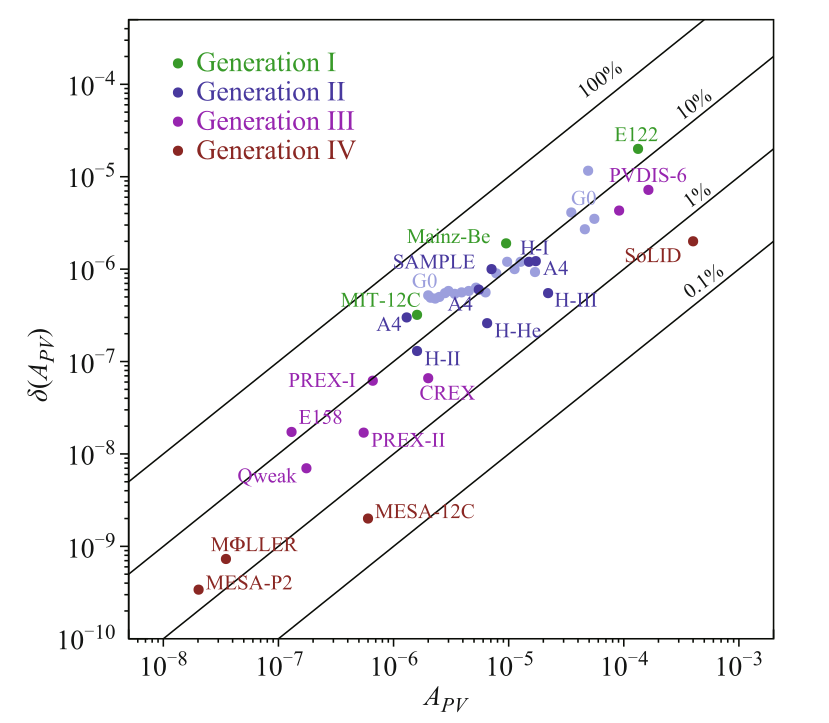
\includegraphics[width=0.5\linewidth]{PVES}
    \caption{Evolution of PVES experiments, solid lines represent the relative 
    precision. Generation I experiments (E122 (1978) \cite{PRESCOTT1978347}, 
    MIT-12C (1989) \cite{PhysRevLett.65.694} and Mainz-Be (1990) \cite{HEIL19891}) 
    did pioneering work to pave the way for PVES. Generation II experiments
    (the SAMPLE collaboration \cite{SAMPLE} at the MIT-Bates accelerator, 
    the G0 \cite{G0} and HAPPEX \cite{HAPPEX} collaboration at Jefferson Lab and
    the A4 collaboration \cite{A4} at the Maizer Mikrotron (MAMI) accelerator) 
    were devoted to the exploration of strange FFs in nucleons.
    Generation III experiments (E158 at SLAC \cite{PhysRevLett.95.081601}, 
    Qweak \cite{PhysRevLett.111.141803} and PVDIS \cite{PhysRevLett.111.082501})
    tested the SM at low energy and measured the neutron skin thickness of nuclei
    (PREX-I/II and CREX). The planned Generation IV experiments (SoLID program \cite{SoLID}
    and M\\OLLER experiment \cite{Moller} at JLab, P2 experiment on the future
    Mainz Energy-recovery Superconducting Accelerator (MESA) \cite{MESA-P2})
    will continue to test the SM and explore the structure of nucleons with higher precisions.
    (MESA-12C is the same experiment as MESA-P2 with a different \C target) }
\end{figure}

Generally, PVES experiments requries 2 experimental conditions: polarized electron
beam and fast flipping of beam polarization. Both requirements actually come to 
the same dependence: an intense source of polarized electrons and with quick response. 
The nature of being PV means measurement between different polarization states, 
while the \textbf{tiny} characteristic of PV asymmetry
demands fast flipping of the polarization states.
To measure such a tiny quantity, it is essential to control
the experimental configurations as the same as possible between different
beam helicities. One obvious and effective method to do the job is to fast 
flipping of beam helicity, the faster the helicity reversal, the smaller
the possible change in beam conditions, target and other apparatus, the smaller
the introduced false asymmetry. This requirement makes PVES out of the capacity
of storage ring accelerators.
% The key for PVES experiments is the fast flipping ($10^2 - 10^3\ Hz$) of beam helicity to reduce 
% the noise caused by fluctuations in target density and the beam qualities, that
% means it is out of the capicity of storage ring accelrators and 
% PVES depends on the development of the intense source of polarized electrons.
Though of the fast reversal of electron's helicity, much effort is needed to
control the beam fluctuation, making it as small as possible. Possible systematic
uncertainties in the source and accelerator will be controlled through the slow
reversal of beam helicity. In terms of the target deformity under electron bombarment,
a raster with very high scanning rate will minimize this uncertainty. As for 
detection of scattered electrons, electron flux rather than single electron will
be counted due to high scattering rate in such experiments.

The 2 sister experiments were conducted in Hall A at JLab, the CEBAF accelerator 
at JLab is one of the few facilities in the world that can do PVES experiments (
other facilities include MIMA and its successor MESA, the Facility for Antiproton
and Ion Research (FAIR) and the Facility for Rare Isotope Beams (FRIB)). CEBAF 
provided excellent polarized electron beams (helicity correlated difference at 
sub-nanometer level) to hall A, with dedicated apparatus 
(Compton polarimeter, taget chamber, HRS and others) in Hall A, we were able 
to measure this tiny asymmetry precisely.

% table of beam parameters
\begin{table}[h]
    \centering
    \begin{tabular}{l | c c }
	\hline
	&   PREX-II & CREX  \\
	\hline
	Target	& \Pb	& \Ca	\\
	Target density ($g/cm^3$)   & 11.38 & 1.855	\\
	Target thickness ($mm$)	& 0.15 + 0.55 + 0.15	& 6	\\
	Number of Target & 10 & 1 + 1	\\
	Used	& 6 & 2	\\
	\hline
	Beam Energy ($GeV$) & 0.953 & 2.18  \\
	Largest Beam Current ($\mu A$)	& 70	& 150	\\
	Average Beam Polarization ($\%$) & 89.7   & 87.1   \\
	Beam Rate ($MHz$) & 249.5	& 249.5 \\
	Electrons/Bunch	($\times 10^6$)	& 1.75	& 3.76	\\
	Helicity Flip Rate ($Hz$)  & 240   & 120   \\
	Power on Target ($Watt$)	&   &	\\
	\hline
	Scattering angle ($\deg$)   & 4.7	& 4.51 \\
	$Q^2$ ($GeV^2$)	& 0.00616   & 0.0297	\\
	Scattering rate ($MHz/arm$)   & 576\footnote{This rate doesn't include the contribution from the diamond foils}   & 13 \\
	xsection ($mbarn$)    & 3930.6	& 5.3   \\
	Acceptance ($msr$)    &	0.0037 & 0.0037  \\
	\hline
	Collected Charge ($C$)	& 114	& 412	\\
	\hline
	predicted $\CA_{pv}$ ($ppm$)	& 0.6   & 2 \\
	proposed precision  & 3.6\%   & 2.4\% \\
	\hline
    \end{tabular}
    \caption{Summary of PREX-II and CREX}
    \label{tb:parameters}
\end{table}

%%%%%%%%%%%%%%%%%%%%%%%%%%%%%%%%%%%%%%%%%%%%%%%%%%%%%%%%%%%%%%%%%%%%%%%%
\section{Kinematics}
PREX-II and CREX are follow-up experiments to PREX-I, which also ran at JLab in 2010. 
With excellent control of systematic uncertainty, but unfortunately, 
many technical challenges during the experiment, PREX-I's result was statistics 
limited, achieving a precision of 10\% \cite{PhysRevLett.108.112502}:
$$ \CA_{Pb} = 656 \pm 60 (stat) \pm 14 (syst) \ ppb$$
Based on the experience and lessons we learned from PREX-I, 
PREX-II and CREX had more well-established designs, which helped to
meet the goal of high-precision.

One important feature of these 2 experiments is the redundancy design for critical
components: we have 2 slow helicity reversal for systematic uncertainty control,
we have 2 polarimeters for polarization measurement, we have multiple BPMs and
BCMs for beam parameter monitoring, we have multiple Pb foil targets and finally
2 HRS arms for electron reception.

%%%%%%%%%%%%%%%%%%%%%%%%
\subsubsection{Uncertainty Budget}
The goal of PREX-II is to achieve the 1\% precision in \Pb neutron radius proposed
by PREX-I, which requires the presicion of PV asymmetry measurement better than 3\%. 
CREX proposed similar goal, that a precision of $0.02 \ fm$ (0.6\%) in the
\Ca neutron radius will be an essential benchmark to test various microscopic 
models, which correspond to a 2.4\% total error in PV asymmetry.

% page 7 in https://prex.jlab.org/DocDB/0000/000065/001/kutz_fom.pdf
As said above, PREX-I already had impressive control over systematic uncertainties (2.1\%),
so will the PREX-II and CREX. The main concern is to collect as much scattered 
electrons as possible to reduce statistical error, which is inversely 
proportional to $\sqrt{N}$.
\begin{table}
    \centering
    \begin{tabular}{c| c c c}
	\hline
	Experiment  & Stat(\%)  & Sys (\%)  & Total (\%)    \\
	\hline
	PREX-II	& 3	& 2	& 3.6	\\ %FIXME: what's the proposed Sys uncertainty
	CREX	& 2.1	& 1.2	& 2.4	\\
	\hline
    \end{tabular}
    \caption{Budget of systematic and statiscal error in both experiments 
    \cite{prex-II_proposal, crex_proposal}
    }
\end{table}

\begin{equation}
    \frac{\delta \CA}{\CA} = \sqrt{\sigma^2_{stat} + \sigma^2_{sys}}	\qquad 
    \sigma_{stat} = \frac{\sigma_{det}}{P\sqrt{N}}
\end{equation}
where:
\begin{itemize}
    \item $\sigma_{det}$ is the detector uncertainty
    \item P is the beam polarizaiton
    \item N is the total number of scattered electrons
\end{itemize}

%%%%%%%%%%%%%%%%%%%%%%%%
\subsection{Figure Of Merits (FOM)}
The choice of beam energy and scattering angle is a compromise of competing
factors. PV asymmetry prefers larger beam energy and larger scattering angle,
while scattering rate falls dramatically with beam energy and scattering angle,
$Q^2$ also likes smaller beam energy and scattering angle, and calculation 
showes that the sensitivity of PV asymmetry w.r.t. neutron radius is oscillating
along beam energy. All these considerations are incorporated into the FOM, which
is defined as:
\begin{equation*}
    \text{FOM} = R \times \CA^2 \times \epsilon^2
\end{equation*}
where R is the scattering rate, $\CA$ the PV asymmetry and $\epsilon$ 
the sensitivity of $\CA$ w.r.t. $R_n$. One difference here is that FOMs for most PVES 
experiments have only R and $\CA^2$, the inclusion of $\epsilon$ in our FOM help
to achieve a higher precision in $R_n$ measurement.

%%%%%%%%%%%%%%%%%%%%%%%%
% from materials/rate_estimation.pdf
\subsubsection{Rate}
For a data set of N independent events sampled from one normal distribution 
$X\sim N(x_0, \sigma_0)$, the statistical uncertainty on the measured mean value
will be:
$$ var(\bar{x} = \frac{1}{n}\sum x_i) = \frac{1}{n^2}var(x_i) = \frac{\sigma_0^2}{n} 
\quad \Longrightarrow \sigma(\bar{x}) = \frac{\sigma_0}{\sqrt{n}} $$

Assume one want to measure a $1 \ ppm$ asymmetry to 1\% statistical uncertainty,
\begin{equation}
    \frac{\sigma_A}{A} = \frac{1}{A}\frac{\sigma_{det}}{\sqrt{2N}} 
    \approx \frac{1}{A\sqrt{2N}} = 1\% \quad 
    \Longrightarrow N = 5 \times 10^{15} 
    \label{eqn:statistical_error}
\end{equation}
a factor of 2 is included because we have 2 HRS arms.
One need to count $\sim10^{15}$ scattered electrons. Given a counting rate of $1\ MHz$, 
it will take $\frac{5\times 10^{15}}{1\ MHz} = 5\times 10^{9}\ s \approx 160 \ years$,
a completely unacceptable time scale. So we have to turn to integrated flux technique
for a higher scattering rate, which is:
\begin{equation}
    \frac{dR(\theta)}{d\Omega} = \frac{d\sigma}{d\Omega}\ I\ t\ \frac{\rho}{A} \times N_A   
\end{equation}
\begin{itemize}
    \item $\frac{d\sigma}{d\Omega}$ is the fractional cross section in $cm^2/str$,
    \item I is the beam current in $electrons/s$
    \item t is the target thickness in $cm$
    \item $\rho$ is the target density in $g/cm^{3}$
    \item A is the atomic number
    \item $N_A = 6.022\times 10^{23}$ is the Avogadro's constant and conversion factors.
\end{itemize}

The differential cross section was numerically calculated by our theoretical friends
with values of $3930.6 \ mbarn$ and $5.3 \ mbarn$ for \Pb and \Ca at their corresponding
kinematics. Other parameters can be checked in table \ref{tb:parameters}.

The total rate will be the integration over the acceptance:
\begin{equation}
    R = \int \frac{dR(\theta)}{d\Omega} d\Omega = \frac{dR}{d\Omega} d\Omega
\end{equation}
PREX-II and CREX have an acceptance defined by the septum and Q1 collimator, which
is $d\Omega = 0.0037 \ str$

Finally, we should also consider radiative correction due to emission of virtual
and real soft photons (Bremsstrahlung), and hard photons by vacuum polarization,
this correction is formulated as:
\begin{equation}
    \eta = \left(\frac{\Delta}{E} \right)^{bt}
\end{equation}
which is evaluated to be: $\eta \sim 0.5$.

\begin{figure}[h!]
    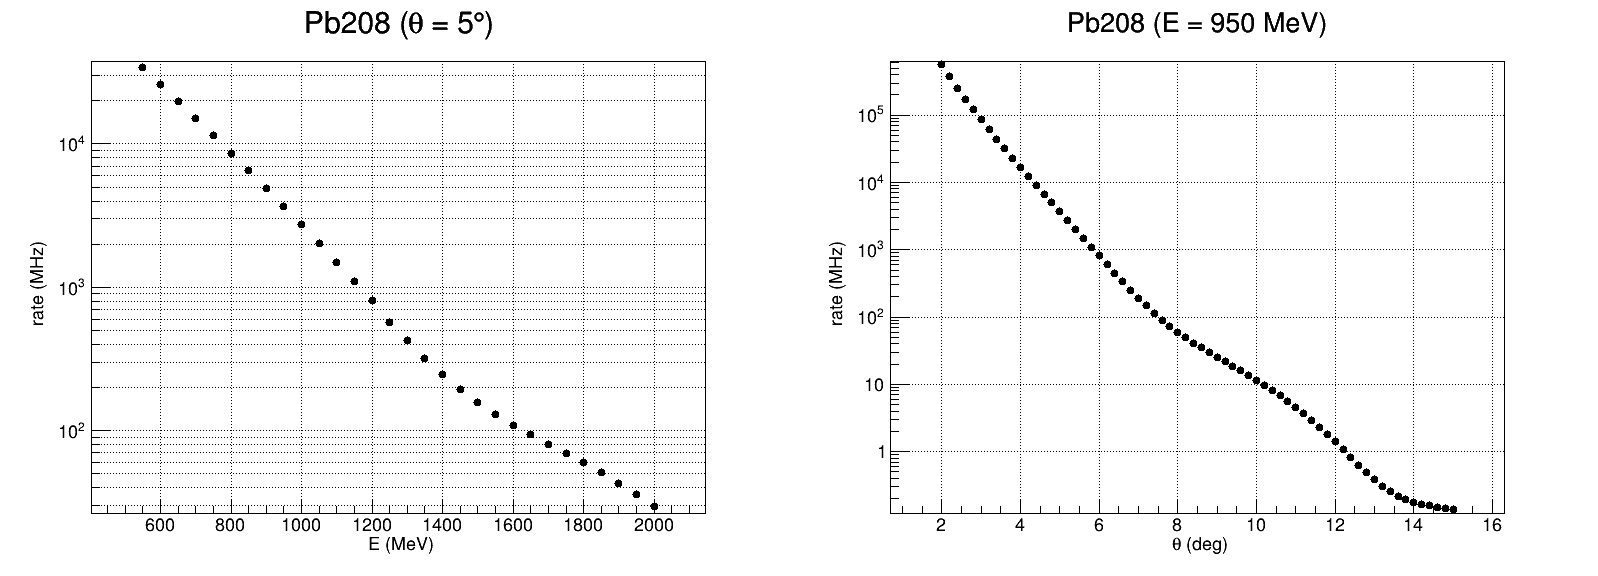
\includegraphics[width=0.5\linewidth]{Pb208_rate}
    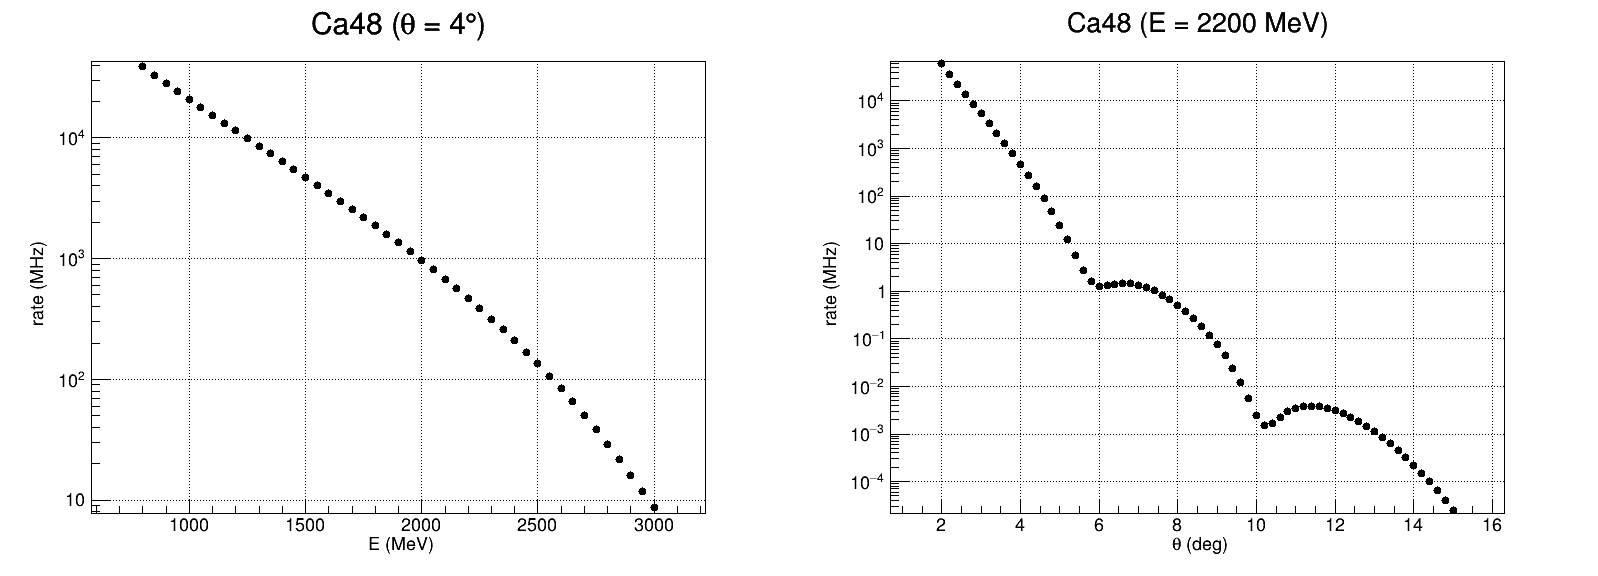
\includegraphics[width=0.5\linewidth]{Ca48_rate}
    \caption{Scattering rate versus beam energy and scattering angle for \Pb and \Ca,
    the energy and scattering angle are design values.
    We see that rate falls quickly along both beam energy and scattering angle for
    both nuclei, so one would like small beam energy and small scattering angle (equivalently
    small $\vec{q}$) for large scattering rate.}
\end{figure}

%%%%%%%%%%%%%%%%%%%%%%%%
\subsubsection{Asymmetry and Sensitivity}
As we shown in eq. \ref{eqn:statistical_error}, the asymmetry itself matters,
a 2 times larger asymmetry means we can reduce the run time to one quarter,
a huge save of beam time. So we should choose the kinematics region where
asymmetry is large. Besides, asymmetry's sensitivity ($\epsilon$) to neutron radius is
also important, keep in mind that our final goal is to extract neutron radius
from PV asymmetry, the more sensitive the asymmetry to neutron radius, the
more precise the extracted neutron radius. The sensitivity is calculated
as the relative change of $\CA$ with 1\% change in neutron radius.
\begin{equation}
    \epsilon = \frac{\delta \CA/\CA}{\delta R/R} = \frac{|\CA_{stretched} - \CA|/\CA}{1\%}
\end{equation}
Though asymmetry is what we want to measure, we can estimate its value based
on some theoretical models, as was numerically calculated by our theoretical 
friends in \cite{PhysRevC.57.3430}.
\begin{figure}[h!]
    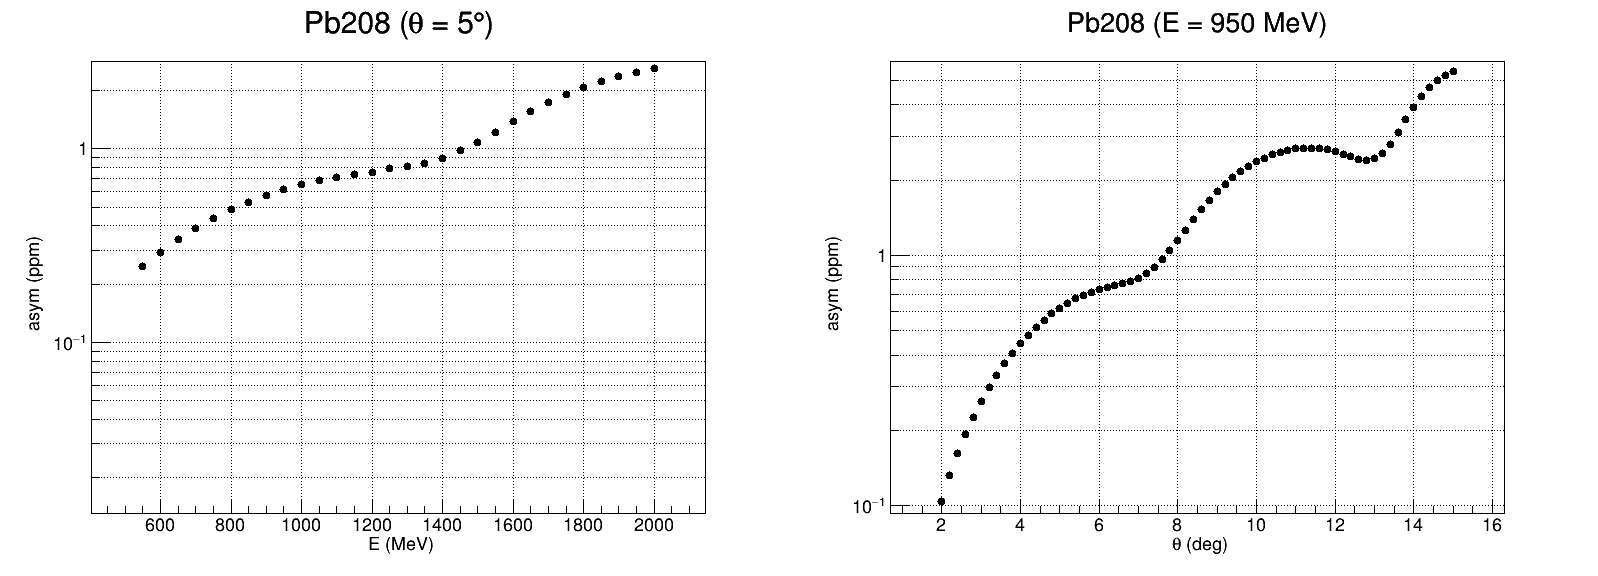
\includegraphics[width=0.5\linewidth]{Pb208_asym}
    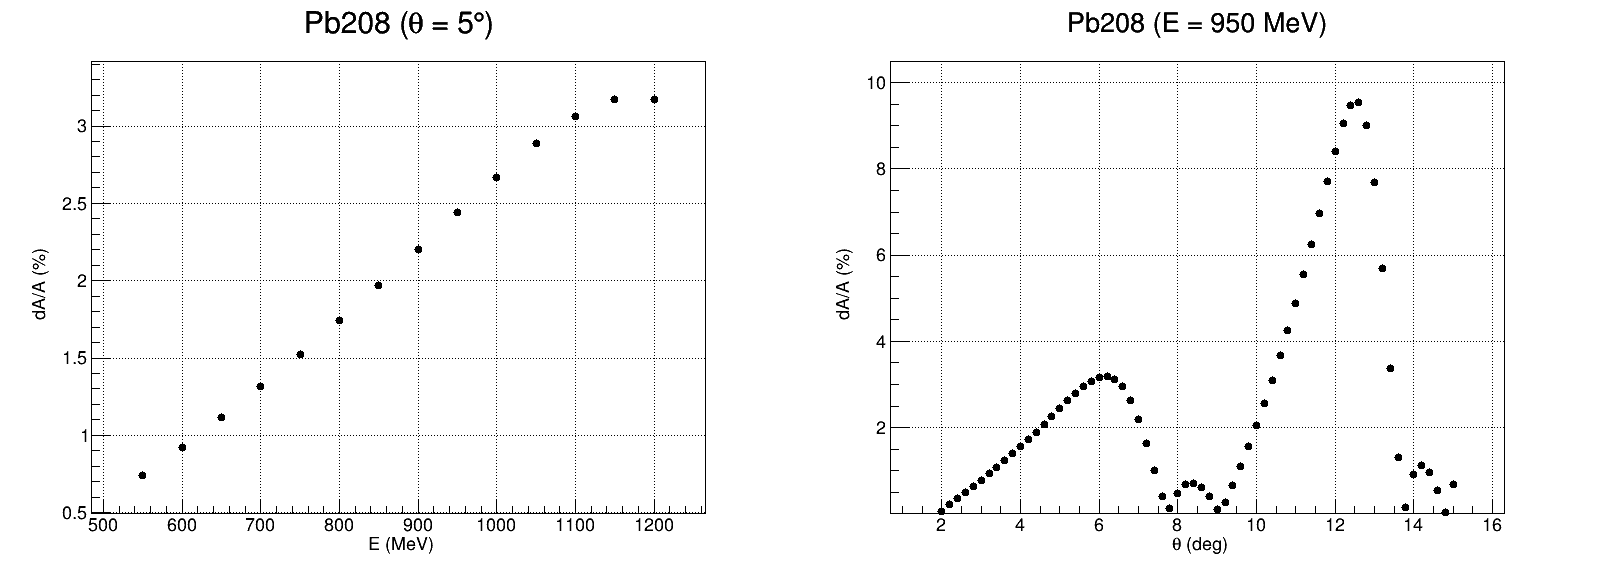
\includegraphics[width=0.5\linewidth]{Pb208_sen}
    \caption{Asymmetry and sensitivity plot for \Pb, which increases along beam 
    energy and oscillating up along scattering angle. The sensitivity plot is
    calculated with 1\% change in neutron radius and it shows the absolute value.
    So in small scattering angle region, there is a local maximum around $6^\circ$}
\end{figure}
\begin{figure}[h!]
    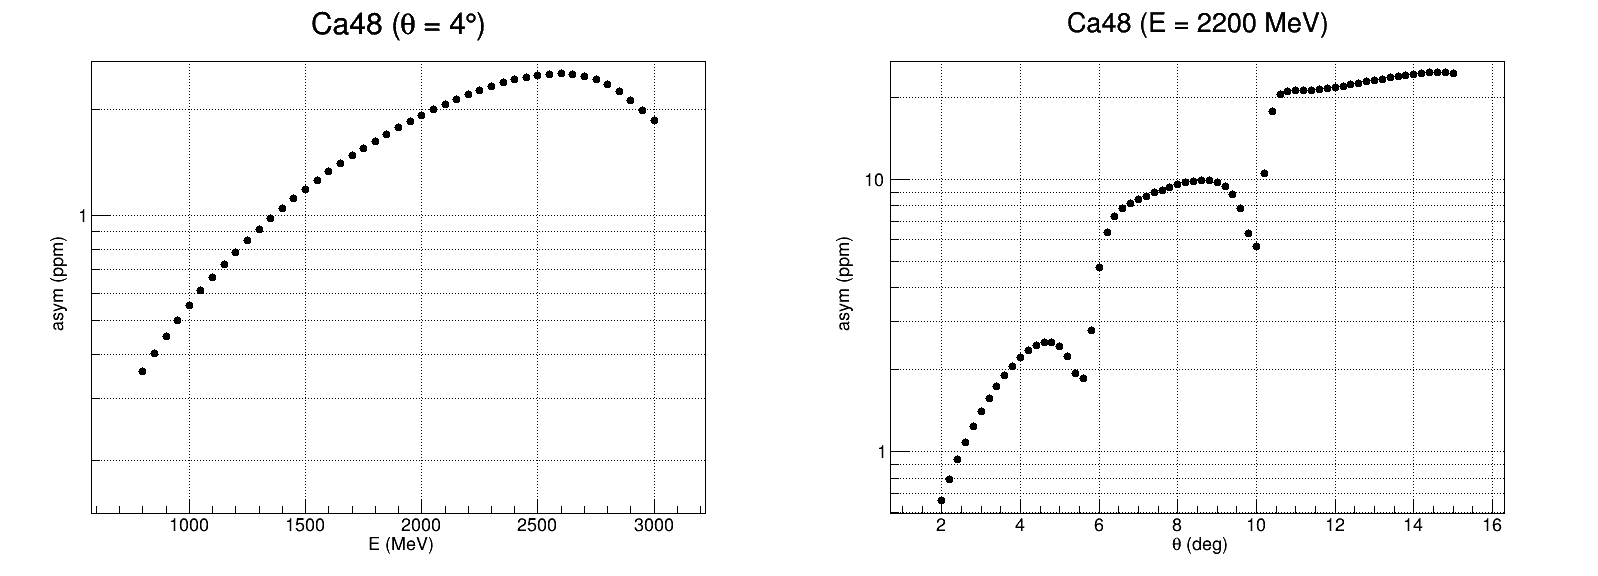
\includegraphics[width=0.5\linewidth]{Ca48_asym}
    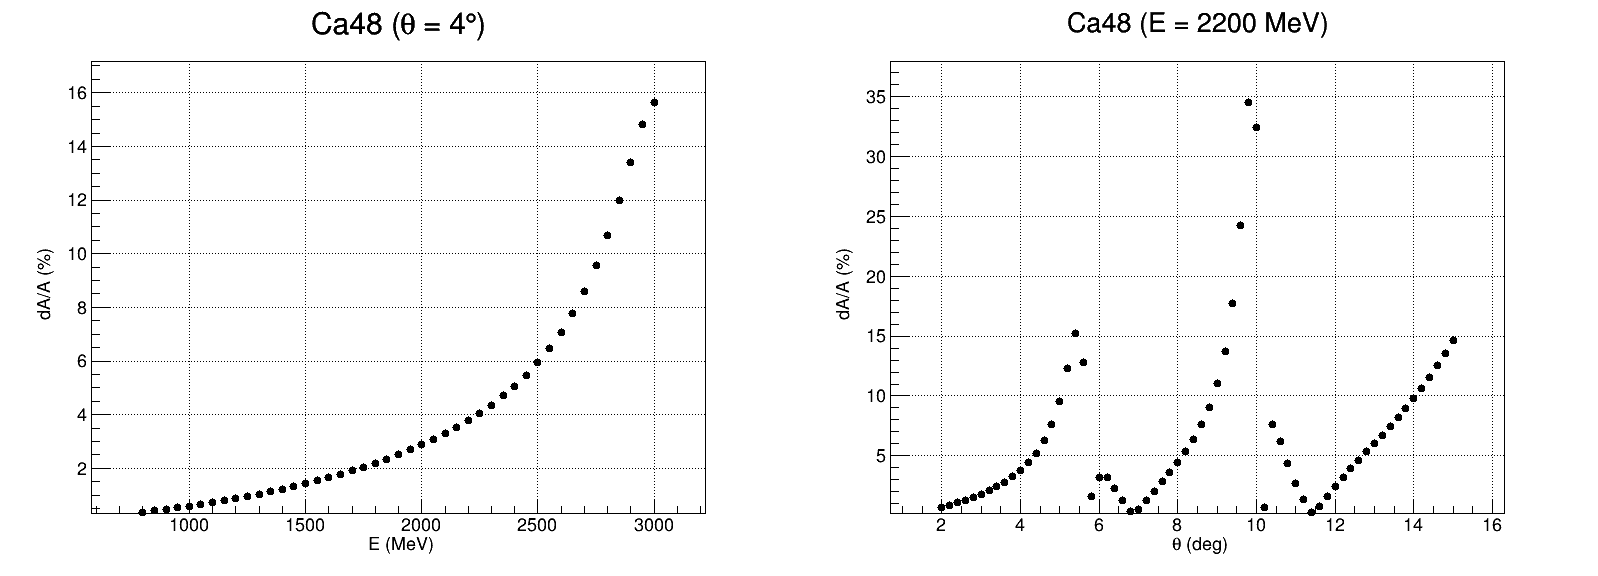
\includegraphics[width=0.5\linewidth]{Ca48_sen}
    \caption{Asymmetry and sensitivity plot for \Ca, the asymmetry maximize around
    2500 MeV and there is a local maximum about $4.5^\circ$. As for sensitivity,
    there is regional maximum around $5^\circ$}
\end{figure}

Based on the theoretical result, we can optimize the kinematics for both nuclei:
\begin{equation}
    \frac{\delta R}{R} = \frac{\delta \CA}{\CA} \frac{1}{\epsilon} 
	= \frac{\sigma_{det}}{P} \frac{1}{\sqrt{N} \CA \epsilon}
\end{equation}
To minimize $\delta R/R$, it is equivalent to maxize 
\begin{equation}
    FOM = N\times \CA^2 \times \epsilon^2
\end{equation}
\begin{figure}
    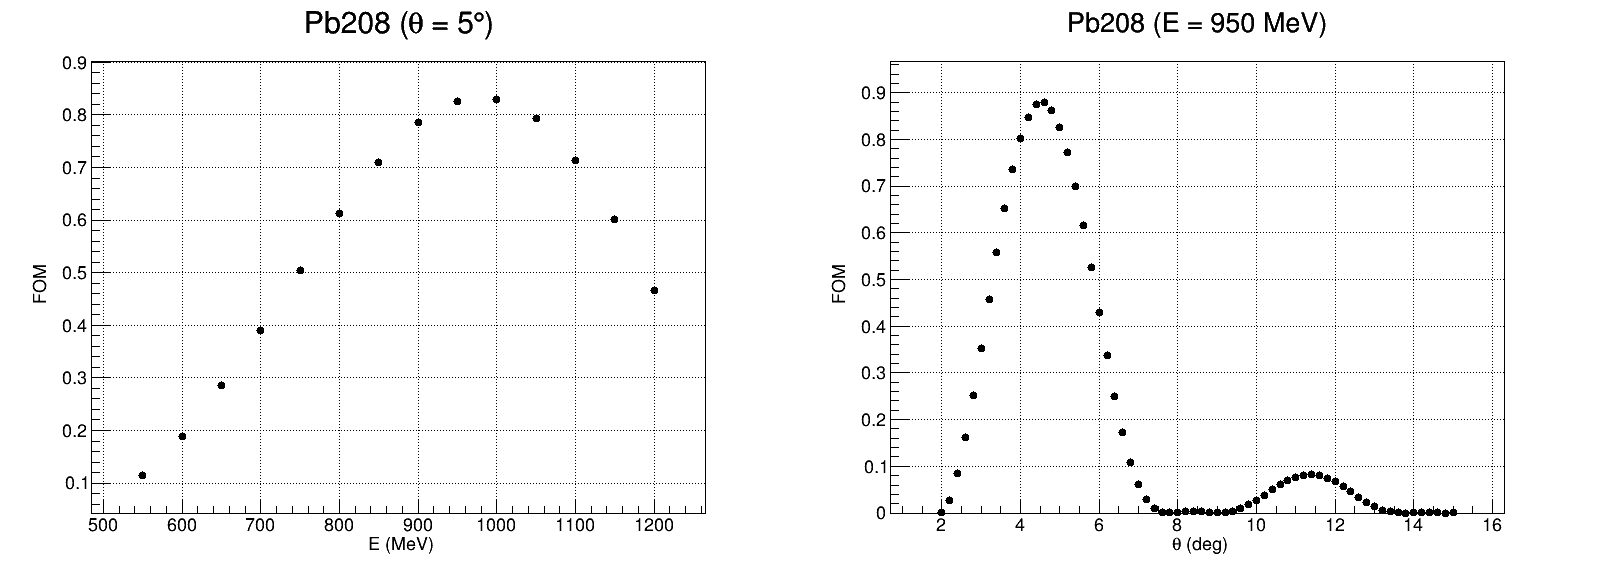
\includegraphics[width=0.5\linewidth]{Pb208_fom}
    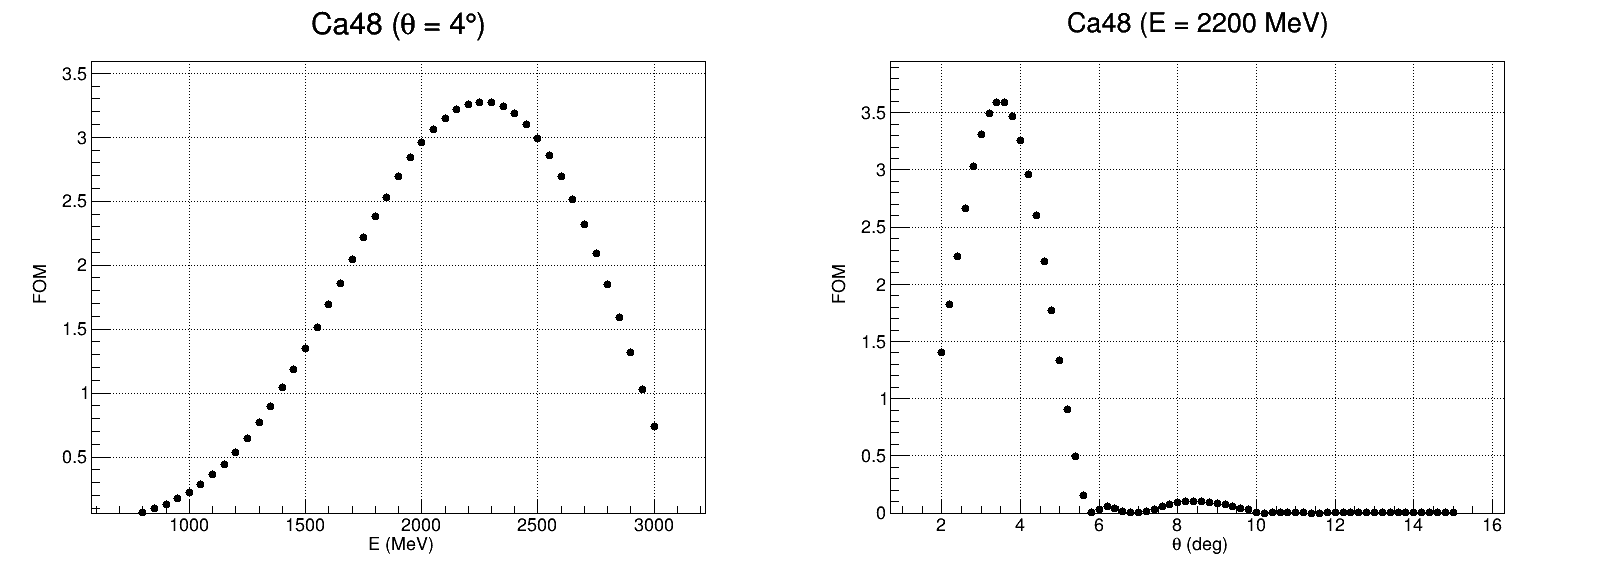
\includegraphics[width=0.5\linewidth]{Ca48_fom}
    \caption{For both nuclei, FOM supports a small scattering angle. As for beam energy,
    FOM maximize around 950 (2200) $GeV$ for \Pb (\Ca).}
\end{figure}

The design values of beam energy and scattering angle were chosed to be 950 (2200) $MeV$
and 5 (4) $degree$ for \Pb (\Ca). The beam energy of CREX is exactly 1-pass beam
energy in CEBAF.
\begin{comment}
    The measured asymmetry will be:
    \begin{equation*}
	\CA = \frac{2\pi}{R} \int \CA_0(\theta)R(\theta)d\theta
    \end{equation*}

    For PREX-II: average sensitivity reduced by 5\% due to ${}^{12}C$ contamination
    For CREX: average sensitivity reduced by 10\% due to ${}^{40}Ca$ contamination

%%%%%%%%%%%%%%%%%%%%%%%%
% \subsubsection{Factor of 1.06}
    While a quartz Cerenkov detector is valued for radiation hardness and insensitivity to soft backgrounds, there is a particular challenge for few GeV electrons. In this energy range, shower fluctuations in a thick or radiated detector significantly degrade energy resolution, while photon statistics degrade the energy resolution for a thin detector. The energy resolution $\Delta E$ at nominal electron energy E increases the statistical error that one would have with infinite resolution $\sigma_0$ to obtain the total statistical error:
$$ \sigma = \sigma_0\sqrt{1+\left(\frac{\Delta E}{E}\right)^2}$$
    
Based on experience in the PREX experiment, we expect an reduction of statistical precision of a factor of 1.06 due to detector resolution.

\bigskip
Using HRS of Hall A, a \textbf{small} scattering angle maximizes the FOM. 
Given practical constraints on how low an angle ($4^\circ$) we can reach with 
septum magnets, the energy is fixed and turns out to be 2.2 GeV, which is a 
natural 1-pass beam energy for CEBAF operations in the 12 GeV era.
\end{comment}

%%%%%%%%%%%%%%%%%%%%%%%%%%%%%%%%%%%%%%%%%%%%%%%%%%%%%%%%%%%%%%%%%%%%%%%%
\section{Continuous Electron Beam Accelerator Facility (CEBAF)}
\begin{figure}[h!]
    \begin{subfigure}[b]{0.59\textwidth}
    \begin{tikzpicture}
	\begin{scope}
	    \node[anchor=south west, inner sep=0] (image) at (0, 0)
	    { 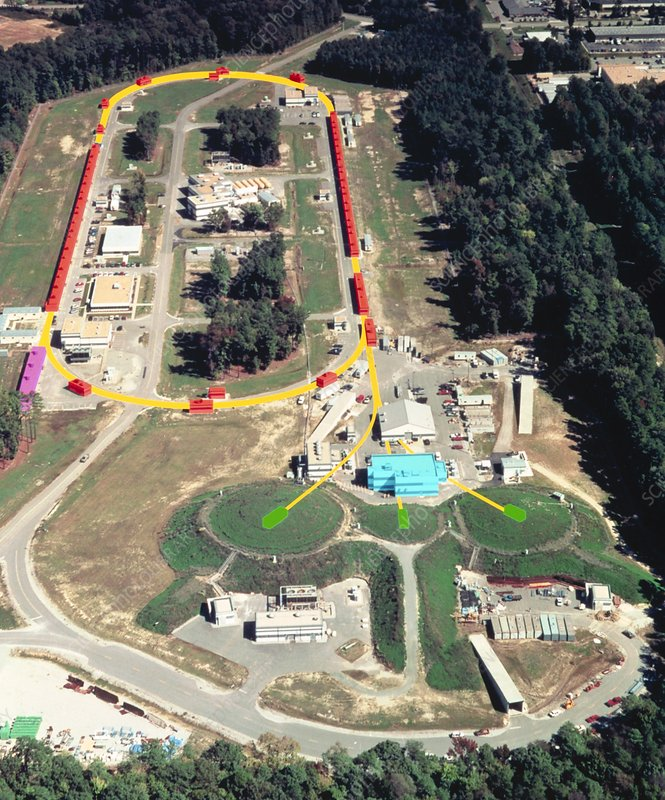
\includegraphics[width=\linewidth]{jlab.jpg} };
	    \begin{scope}[x={(image.south east)}, y={(image.north west)}]
		\node [red] at (0.415, 0.355) {\textbf{A}};
		\node [red] at (0.610, 0.355) {\textbf{B}};
		\node [red] at (0.780, 0.355) {\textbf{C}};
	    \end{scope}
	\end{scope}
    \end{tikzpicture}
    \end{subfigure}
    \begin{subfigure}[b]{0.5\textwidth}
	\includegraphics[width=0.9\linewidth]{tunnel_construction}
	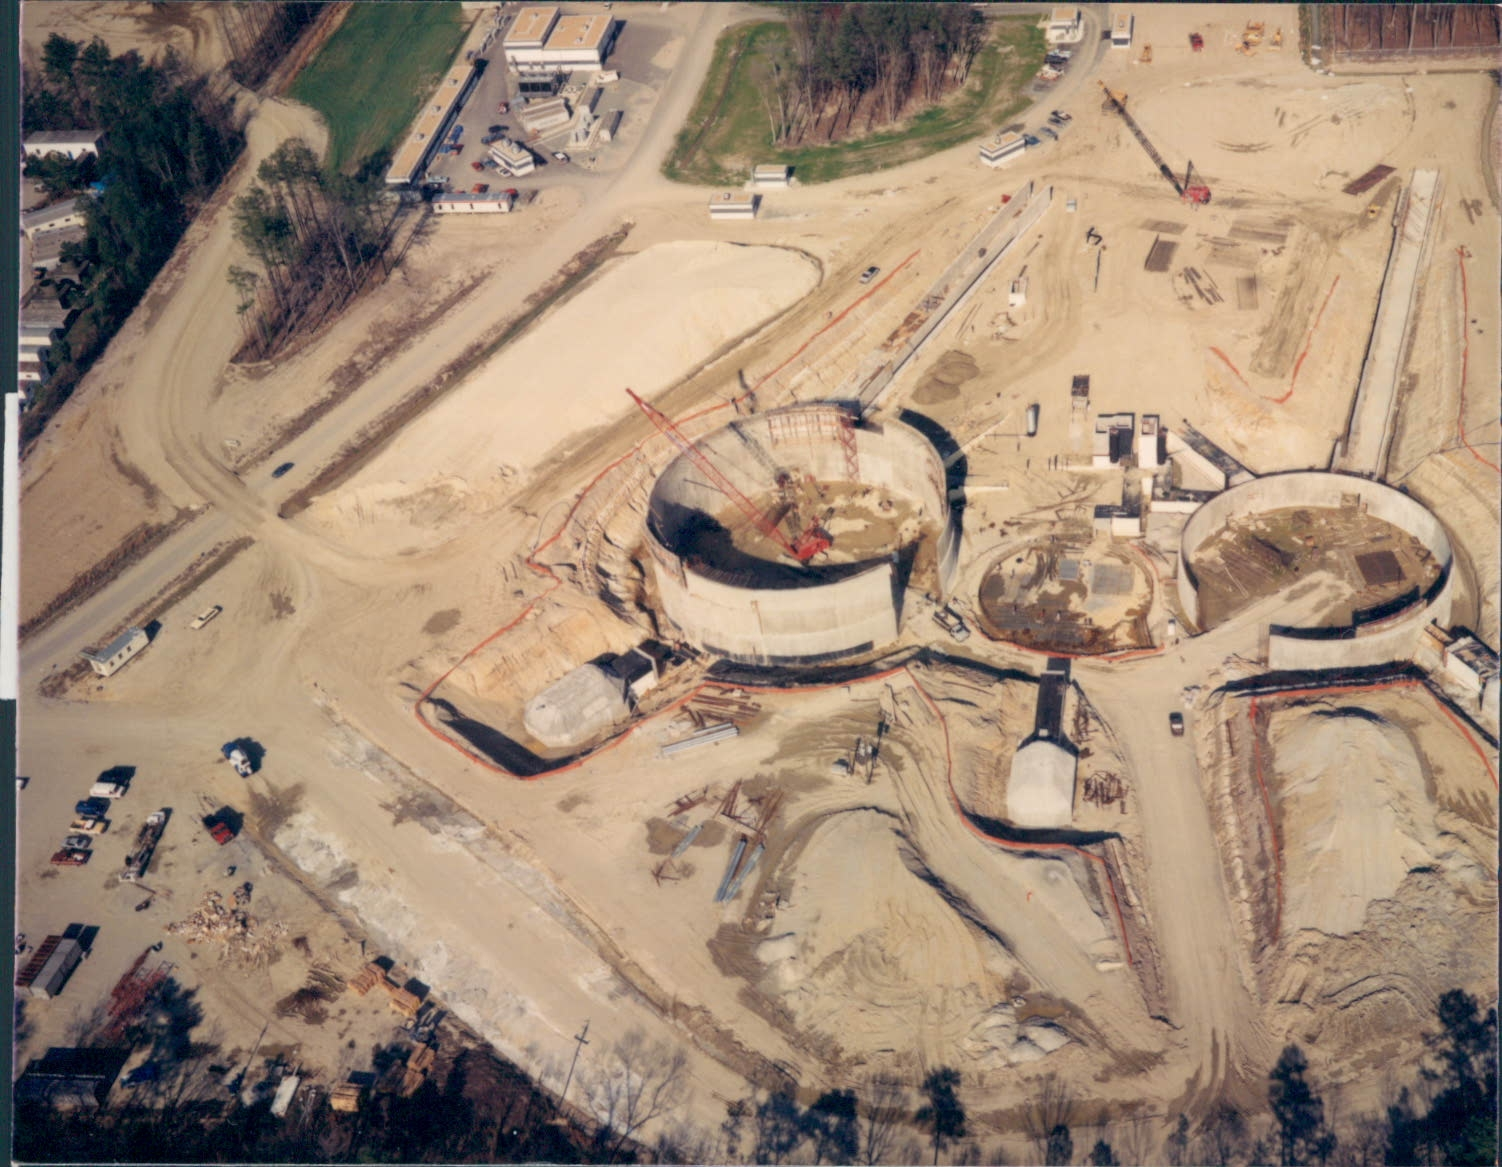
\includegraphics[width=0.9\linewidth]{hall_construction}
    \end{subfigure}

    \caption{Aerial view of JLab accelerator site, yellow line tells the position
    of the CEBAF accelerator and the 3 experimental halls are marked out as A/B/C 
    (Hall D locates on the top left corner, after the exit of north LINAC).
    The accelerator tunnel is $30 \ feet$ ($\sim 9 \ m$) underground and $10 \ feet$ ($\sim 3 \ m$) 
    high, with a circumference of about $7/8\ miles$ ($1.4\ km$). There are 2 superconducting 
    LINAC (red lines), each of $1/4\ miles$ ($400\ m$). The pink part on the mid
    left is the location of injector. The right 2 plots show the tunnel and 
    experimental halls under construction.}
\end{figure}

\begin{figure}[h!]
    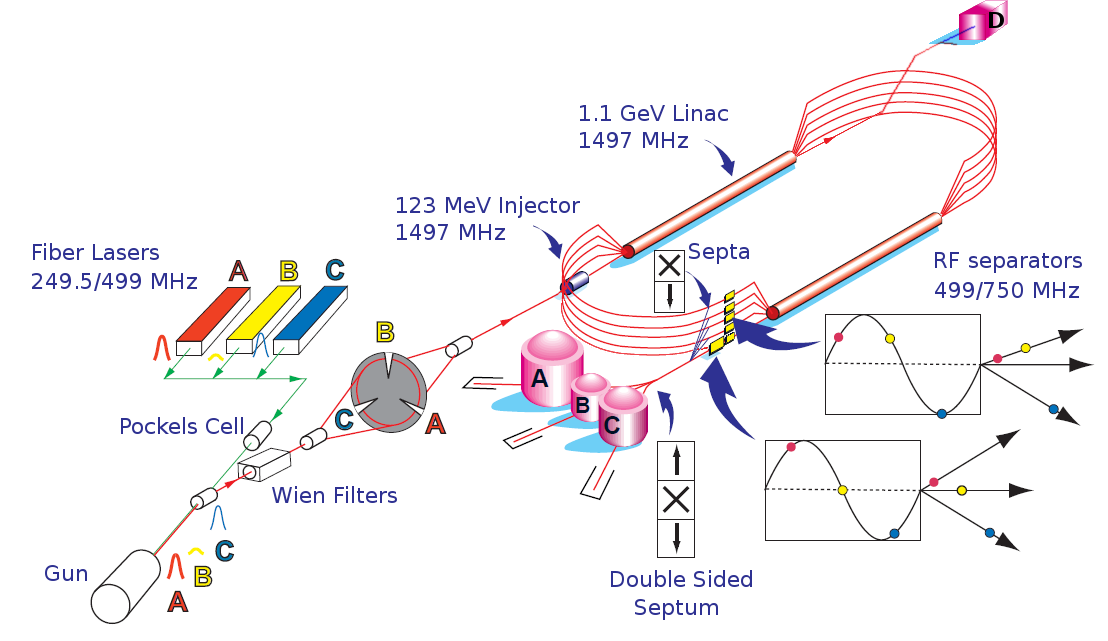
\includegraphics[width=0.9\linewidth]{cebaf.png}
    \caption{Schematic plot of CEBAF. Low energy beams will be kicked into 
    higher arc, and high energy beams will go through lower arc. The magnetic
    field increases from higher arc to lower arc to keep electron trajectory 
    have the same radius.}
    \label{fig:cebaf}
\end{figure}
CEBAF is able to deliver multi-GeV continuous wave (cw) eletron beams of different
energies and different intensities to 4 halls simultaneously.
With the 12 GeV upgrade, the north and south $1497\ MHz$ LINAC each has 25 
Superconducting Radial Frequency (SRF) cryomodules, capable of accelrating 
electrons at the peak rate of 2.2 $GeV/turn$. Hall A, B and C can receive up
to $2.2 \times 5 = 11 \ GeV$ cw beams and Hall D, with an extra half circle,
can receive up to $12\ GeV$ cw beams. With this design, different nuclear 
experiments can be carried out in different halls without interfering each other,
theoretically.

As one can see in \ref{fig:cebaf}, laser pulse from 4 lasers (Hall D laser is not
shown in the plot) shoot in the electron gun (2 electron guns in total) that 
operates at $-130\ kV$ to excite electrons, which interweaving with each other, 
forming a chain of electron bunches, with a phase difference of $120^\circ$ from 
neaby bunches (Hall D doesn't have its own slit in the chopper, therefore 
it follows either Hall A or Hall C). This electron chain is sent into north LINAC
by the injector, accelerated by both LINACs. After reaching desired energy,
they will be kicked out at the exit of south LINAC and delivered to experimental
halls (A, B and C) for various experiments. 

The maxium beam current of $200\ \mu A$ at (old) highest energy of $5\ GeV$ 
available at CEBAF is limited by the rf power ($1\ MW = 5\ GeV \times 200\ \mu A$) 
and by the beam power on the beam dump. While Hall B and D requires only tiny 
amount of cw beams (at $nA$ level), it is actually Hall A and C that consume 
the produced electron beams, both can receive a few tenths to over one 
hundred $\mu A$.

While all 4 halls at JLab are dedicated to the study of nuclear structure, they
focus on different aspects. Hall A concentrates on form factors of various nuclei, 
Hall B digs into generalized parton distributions, Hall C devotes itself to precise
determination of valance quark properties in nuclei, and finally, the newly 
established Hall D explores origin of confinement through exotic mesons.

Because all 4 halls shared the same electron source and the same accelerator, 
cooperation is needed to make them work at the same time. In terms of electron
source, PVES experiment usually has priority over other experiments to maintain 
the quality of polarized electron beam. As for the LINAC, if one hall wants
a smaller energy, say $1\ GeV$, then the LINAC power will be reduced to $1\ GeV/turn$,
which will be applied to other halls' electron beams, therefore limiting the 
highest energy available in other halls. Careful schedule is needed to make sure
every hall get what they want.
%%%%%%%%%%%%%%%%%%%%%%%%%%%%%%%%%%%%%%%%%%%%%%%%%%%%%%%%%%%%%%%%%%%%%%%%
\section{Polarized Electron}
% The key to the success of this experiment was the 1975 discovery of a new method for producing
% polarized electrons made by a group in Colorado, which included E.L. Garwin of SLAC.
% Shortly thereafter, a new source was built for the SLAC linac utilizing the method, thus
% allowing for the 1978 parity violation measurements which were in close agreement with
% those predicted by the GWS model. 

%%%%%%%%%%%%%%%%%%%%%%%%%%%%%%%%%%%%%%%%%%%%%%%%
\subsection{Polarized Electron Source}
PVES experiments motivate the development of polarized electron source, which 
require a highly stable polarized electron source that can produce
high polarization electron beam at a wide range of intensity, from nA to A 
depending on the experiment. The source should be capable of rapid helicity
reversal ($\sim 100 Hz$) with negligible impact on other properties of the beam.

Currently, GaAs-based semiconductor photoemission source is % confirmed by Wang Yan
the only available polarized electron source for accelerators on the market.
Historically, this 
kind of electron source was the only one that could satisfy high peak currents 
required by the low duty factors of the old accelerators and rapid helicity 
reversal required by PVES. That's why it is the only player on the market now.
Over the past few decades, pulsed beam has been replaced by continuous beam while
this electron source is inheritated and further developed. The polarized electron
source used by CEBAF can produce electron beam with polarization greater than
85\%, much larger than the 37\% polarization from its inauguration at SLAC. \cite{PRESCOTT1978347}

The design was first proposed independently by Garwin, Pierce and Siegmann \cite{GARWIN}
and by Lampel and Weisbuch \cite{LAMPEL1975877}. The idea is straightforward:
When circularly polarized laser light with carefully selected energy $E_{gap} < h\nu < E_{gap} + \Delta$
shoot on the semiconductor, only electrons on the valance band $P_{3/2}$ will be
pumped into the conduction band $S_{1/2}$. The selection rule makes sure only
those transitions that satisfy $\Delta m_j = +1 \ (-1)$ can occur for circularly
right (left) incoming photons, As shown in fig. \ref{fig:excitation-b}.
The ratio of the transition rate is also marked out in circle in the plot, 
which can be calculated from the Clebsch-Gordan coefficient easily. The excited
electrons are polarzied and different states have different pumping rate, so
we have polarized electron beam now with polarization as: P = (3-1)/(3+1) = 50\%,
for both cases.
\begin{figure}[h!]
    \tikzmath{\yone=1.3; \ytwo=2.5; \ythree=5;} 
    \centering
    \begin{subfigure}[b]{0.49\textwidth}
	\centering
	\begin{tikzpicture}
	    \centering
	    \begin{axis}[axis lines=middle,
		xmin=-1.4, xmax=2.75,
		ymin=0, ymax=7,
		xlabel={\large $k$},
		ylabel={\large$E$},
		xlabel style={below},
		xtick=\empty,
		ytick=\empty,
		x axis line style={draw=none},
		% clip=false,
		]
		\addplot[Violet, line width=3pt, samples=100, domain=-0.7:0.7, name path=A] {-2*x^2 + \yone};
		\addplot[OliveGreen, line width=3pt, samples=100, domain=-0.7:0.7, name path=B] {-2*x^2 + \ytwo};
		\addplot[OliveGreen, line width=3pt, samples=100, domain=-0.7:0.7, name path=B] {-1.2*x^2 + \ytwo};
		\addplot[Blue, line width=3pt, samples=100, domain=-0.7:0.7, name path=B] {2*x^2 + \ythree};
		\draw [/pgfplots/every inner x axis line, draw=black] (0,0) -- (\pgfkeysvalueof{/pgfplots/xmax}, 0); 
		\draw [dashed, draw=black] (0,\yone) -- (\pgfkeysvalueof{/pgfplots/xmax}, \yone);
		\draw [dashed, draw=black] (0,\ytwo) -- (\pgfkeysvalueof{/pgfplots/xmax}, \ytwo);
		\draw [dashed, draw=black] (0,\ythree) -- (\pgfkeysvalueof{/pgfplots/xmax}, \ythree);
		\draw [stealth-stealth, thick] (0.8, \yone) -- (0.8, \ytwo) node [midway, right] {\bm{$\Delta = 0.34\ eV$}};
		\draw [stealth-stealth, thick] (0.8, \ytwo) -- (0.8, \ythree) node [midway, right] {\bm{$E_{gap} = 1.42\ eV$}};
		\node [Violet, below] at (-1, \yone) {\large\bm{$P_{1/2}$}};
		\node [OliveGreen, below] at (-1, \ytwo) {\large\bm{$P_{3/2}$}};
		\node [Blue, above] at (-1, \ythree) {\large\bm{$S_{1/2}$}};
		\node [left, above] at (-0.2, \ytwo) {\large\bm{$E_F$}};
	    \end{axis}
	    \label{fig:excitation-a}
	\end{tikzpicture}
    \end{subfigure}
    \hfill
    \begin{subfigure}[b]{0.49\textwidth}
	\centering
	\begin{tikzpicture}
	    \begin{axis}[axis lines=middle,
		xmin=0, xmax=8,
		ymin=0, ymax=7,
		xlabel={\large $m_j$},
		ylabel={\large$E$},
		xlabel style={below},
		xtick=\empty,
		ytick=\empty,
		]
		\draw [/pgfplots/every inner y axis line, draw=black] (6.5,0) -- (6.5, \pgfkeysvalueof{/pgfplots/ymax}) node [below right] {\large J}; 
		\draw [draw=Violet, line width=2pt] (1.25,\yone) -- (2.25, \yone) node [midway, below, Violet] {\textbf{-1/2}};
		\draw [draw=Violet, line width=2pt] (4.25,\yone) -- (5.25, \yone) node [midway, below, Violet] {\textbf{+1/2}};
		\draw [draw=OliveGreen, line width=2pt] (0.5,\ytwo) -- (1.5, \ytwo) node [midway, below, OliveGreen] {\textbf{-3/2}};
		\draw [draw=OliveGreen, line width=2pt] (2,\ytwo) -- (3, \ytwo) node [midway, below, OliveGreen] {\textbf{-1/2}};
		\draw [draw=OliveGreen, line width=2pt] (3.5,\ytwo) -- (4.5, \ytwo) node [midway, below, OliveGreen] {\textbf{+1/2}};
		\draw [draw=OliveGreen, line width=2pt] (5,\ytwo) -- (6, \ytwo) node [midway, below, OliveGreen] {\textbf{+3/2}};
		\draw [draw=Blue, line width=2pt] (2,\ythree) -- (3, \ythree) node [midway, above, Blue] {\textbf{-1/2}};
		\draw [draw=Blue, line width=2pt] (3.5,\ythree) -- (4.5, \ythree) node [midway, above, Blue] {\textbf{+1/2}};
		\node [Violet, right] at (6.7, \yone-0.1) {\large\bm{$P_{1/2}$}};
		\node [OliveGreen, right] at (6.7, \ytwo-0.1) {\large\bm{$P_{3/2}$}};
		\node [Blue, right] at (6.7, \ythree-0.1) {\large\bm{$S_{1/2}$}};

		\draw [-stealth, Red, line width=2pt] (1, \ytwo) -- (2.5, \ythree) node [midway, circle, fill=CornflowerBlue, text=Black] {\textbf{3}};
		\draw [-stealth, Red, line width=2pt] (2.5, \ytwo) -- (4, \ythree);
		\node [above, Red] at (1, \ytwo+0.5) {\bm{$\sigma^+$}};
		\draw [-stealth, YellowOrange, line width=2pt] (4, \ytwo) -- (2.5, \ythree) node [midway, circle, fill=CornflowerBlue, text=Black] {\textbf{1}};
		\draw [-stealth, YellowOrange, line width=2pt] (5.5, \ytwo) -- (4, \ythree) node [midway, circle, fill=CornflowerBlue, text=Black] {\textbf{3}};
		\node [above, YellowOrange] at (5.5, \ytwo+0.5) {\bm{$\sigma^-$}};
	    \end{axis}
	\end{tikzpicture}
	\label{fig:excitation-b}
    \end{subfigure}
    \caption{Excitation of polarized electrons}
\end{figure}

\begin{figure}[h!]
    \centering
    \begin{subfigure}[b]{0.32\textwidth}
	\tikzmath{\yone=2.5; \ytwo=5; \ythree=9.5;} 
	\centering
	\resizebox{\textwidth}{0.33\textheight}{
	\begin{tikzpicture}
	    \centering
	    \begin{axis}[
		axis lines=middle,
		xmin=-3, xmax=1,
		ymin=0, ymax=10,
		hide axis,
		]
		\draw [dashed] (\pgfkeysvalueof{/pgfplots/xmin}, \yone) -- (0, \yone) node [right] {\bm{$E_F$}};
		\draw [dashed] (\pgfkeysvalueof{/pgfplots/xmin}, \ytwo) -- (0, \ytwo);
		\draw [dashed] (\pgfkeysvalueof{/pgfplots/xmin}, \ythree) -- (0, \ythree);
		\draw [Violet, line width=2pt] (0, 0) -- (0, \ythree) -- (\pgfkeysvalueof{/pgfplots/xmax}/4, \ythree) node [right, Black] {\bm{$E_\infty$}};
		\fill [pattern=north east lines] (\pgfkeysvalueof{/pgfplots/xmin}, \yone)  -- (-1, \yone) arc (90:0:1) -- (0, 0) -- (\pgfkeysvalueof{/pgfplots/xmin}, 0) -- (\pgfkeysvalueof{/pgfplots/xmin}, \yone);
		\draw [Violet, line width=2pt] (\pgfkeysvalueof{/pgfplots/xmin}, \yone)  -- (-1, \yone) arc (90:0:1);
		\draw [Violet, line width=2pt] (\pgfkeysvalueof{/pgfplots/xmin}, \ytwo)  -- (-1, \ytwo) arc (90:0:1);
		\draw [stealth-stealth, thick] (\pgfkeysvalueof{/pgfplots/xmin} + 0.8, \yone) -- (\pgfkeysvalueof{/pgfplots/xmin} + 0.8, \ytwo) node [midway, left] {\bm{$E_{gap}$}};
		\draw [stealth-stealth, thick, Red] (-0.5, \ytwo) -- (-0.5, \ythree) node [midway, left] {\textbf{PEA = 4.07 eV}};
		\node [Red, above] at (\pgfkeysvalueof{/pgfplots/xmin}/2, 0) {\textbf{GaAs}};
		\node [Red, above right] at (0, 0) {\textbf{Vac}};
		\node [below left, text width=2cm] at (-0.5, \yone) {\textbf{Valance Band}};
		\node [below left, text width=2cm] at (-0.5, \ytwo) {\textbf{Conduction Band}};
	    \end{axis}
	\end{tikzpicture}
	}
	\label{fig:PEA}
    \end{subfigure}
    \hfill
    \begin{subfigure}[b]{0.32\textwidth}
	\tikzmath{\yone=2.5; \ytwo=5; \ythree=9.5;} 
	\centering
	\resizebox{\textwidth}{0.33\textheight}{
	\begin{tikzpicture}
	    \centering
	    \begin{axis}[
		axis lines=middle,
		xmin=-3, xmax=1,
		ymin=0, ymax=10,
		hide axis,
		]
		\draw [dashed] (\pgfkeysvalueof{/pgfplots/xmin}, \yone) -- (0, \yone) node [right] {\bm{$E_F$}};
		\draw [dashed] (\pgfkeysvalueof{/pgfplots/xmin}, \ytwo) -- (0, \ytwo);
		\node at (0, \pgfkeysvalueof{/pgfplots/ymax}) {};
		\draw [OliveGreen, line width=5pt] (-0.07, 0) -- (-0.07, \ytwo);
		\draw [Violet, line width=2pt] (0, 0) -- (0, \ytwo) -- (\pgfkeysvalueof{/pgfplots/xmax}/4, \ytwo) node [right, Black] {\bm{$E_\infty$}};
		\fill [pattern=north east lines] (\pgfkeysvalueof{/pgfplots/xmin}, \yone)  -- (-1, \yone) arc (90:0:1) -- (0, 0) -- (\pgfkeysvalueof{/pgfplots/xmin}, 0) -- (\pgfkeysvalueof{/pgfplots/xmin}, \yone);
		\draw [Violet, line width=2pt] (\pgfkeysvalueof{/pgfplots/xmin}, \yone)  -- (-1, \yone) arc (90:0:1);
		\draw [Violet, line width=2pt] (\pgfkeysvalueof{/pgfplots/xmin}, \ytwo)  -- (-1, \ytwo) arc (90:0:1);
		\node [Red, above] at (\pgfkeysvalueof{/pgfplots/xmin}/2, 0) {\textbf{GaAs}};
		\node [Red, above] at (-0.03, 0) {\textbf{Cs}};
		\node [Red, above right] at (0.1, 0) {\textbf{Vac}};
	    \end{axis}
	\end{tikzpicture}
	}
	\label{fig:ZEA}	% zero EA
    \end{subfigure}
    \hfill
    \begin{subfigure}[b]{0.32\textwidth}
	\tikzmath{\yone=2.5; \ytwo=5; \ythree=4; \surface=0.8;} 
	\centering
	\resizebox{\textwidth}{0.33\textheight}{
	\begin{tikzpicture}
	    \centering
	    \begin{axis}[
		axis lines=middle,
		xmin=-3, xmax=1,
		ymin=0, ymax=10,
		hide axis,
		]
		\draw [dashed] (\pgfkeysvalueof{/pgfplots/xmin}, \yone) -- (0, \yone) node [right] {\bm{$E_F$}};
		\draw [dashed] (\pgfkeysvalueof{/pgfplots/xmin}, \ytwo) -- (0, \ytwo);
		\draw [dashed] (\pgfkeysvalueof{/pgfplots/xmin}, \ythree) -- (0, \ythree);
		\node at (0, \pgfkeysvalueof{/pgfplots/ymax}) {};
		\draw [Violet, line width=2pt] (0, 0) -- (0, \ythree) -- (\pgfkeysvalueof{/pgfplots/xmax}/4, \ythree) node [right, Black] {\bm{$E_\infty$}};
		\fill [pattern=north east lines] (\pgfkeysvalueof{/pgfplots/xmin}, \yone)  -- (-1-\surface, \yone) arc (90:0:1) -- (-\surface, 1.4) arc (180:270:\surface) --  (0, 0) -- (\pgfkeysvalueof{/pgfplots/xmin}, 0) -- (\pgfkeysvalueof{/pgfplots/xmin}, \yone);
		\draw [Violet, line width=2pt] (-\surface, 0) -- (-\surface, \ytwo/2 + \ythree/2) arc (180:270:\surface);
		\draw [Violet, line width=2pt] (-\surface, 1.4) arc (180:270:\surface);
		\draw [Violet, line width=2pt] (\pgfkeysvalueof{/pgfplots/xmin}, \yone)  -- (-1-\surface, \yone) arc (90:0:1);
		\draw [Violet, line width=2pt] (\pgfkeysvalueof{/pgfplots/xmin}, \ytwo)  -- (-1-\surface, \ytwo) arc (90:0:1);
		\node [Red, above] at (\pgfkeysvalueof{/pgfplots/xmin}/2, 0) {\textbf{GaAs}};
		\node [Red, above] at (-0.4, 0) {\bm{$Cs_2O$}};
		\node [Red, above right] at (0.1, 0) {\textbf{Vac}};

		\node (e1) at (\pgfkeysvalueof{/pgfplots/xmin}/5*3, \yone)[circle, fill=CornflowerBlue, text=Black] {\textbf{e}};
		\node (e2) at (\pgfkeysvalueof{/pgfplots/xmin}/5*3, \ytwo)[circle, fill=CornflowerBlue, text=Black] {\textbf{e}};
		\node (e3) at (0.2, \ythree*1.1)[circle, fill=CornflowerBlue, text=Black] {\textbf{e}};
		\draw [-stealth, thick, CornflowerBlue] (e1) -- (e2);
		\draw [-stealth, thick, CornflowerBlue] (e2) -- (e3);
		\draw [stealth-stealth, thick, Red] (-2.2, \ytwo) -- (-2.2, \ythree) node [midway, left] {\textbf{NEA}};
	    \end{axis}
	\end{tikzpicture}
	}
	\label{fig:NEA}
    \end{subfigure}
    \caption{The energy band diagram of GaAs near its surfacer. 
    Left: bare p-type GaAs, the large positive electron affinity (PEA) 
    prevents electrons from escaping the surface; 
    Middle: p-type GaAs with a cesiated surface, the electron affinity (EA)
    is 0, but electrons still can't escape the surface easily; 
    Right: GaAs with layer of cesium oxide; the electron vaccum energy $E_\infty$ is
    lowered to make a negative EA so that electrons can break free the surface
    easily. \cite{CARDMAN1992317}}
\end{figure}
Then how can we liberate the polarzied electrons from the material, without 
degenerating the polarization significantly. As shown in fig. \ref{fig:PEA},
for bare GaAs, a $4.07 ev$ electron affinity (EA) prevents any electrons from
leaving the surface. To solve this problem, a condition known as negative
electron affinity (NEA) is used, that is to make the energy of electron in 
the vaccum just outside the surface lower than the conduction band energy by
adding a layer a cesium oxide on the surface of pure GaAs semiconductor.

By the NEA technique, we were able to get polarized electron beam, but never
reached the ideal 50\% polarization, achieved polarization range between 25 to 43\%
. The polarization loss is due to spin dilution as electrons diffuse to the 
semiconductor surface. From this aspect, we can increase the polarization by 
reducing the thickness of the GaAs crystal. But obviously, even the thinnest
GaAs crystal can't give us a polarization greater than 50\%. New strategies 
are needed. It turned out the answer was strained GaAs. \cite{CARDMAN1992317}

With a strained layer, the degeneracy of $P_{3/2}$ state is splitted, 
only states with $m_j = \pm 3/2$ will be pumped, therefore we will get 100\% 
polarization, in ideal case. The real polaration achieved by CEBAF electron
source is about 88\%.
\begin{figure}[h!]
    \tikzmath{\yone=1.3; \ytwo=2.5; \ythree=5;} 
    \centering
    \begin{subfigure}[b]{0.49\textwidth}
	\centering
	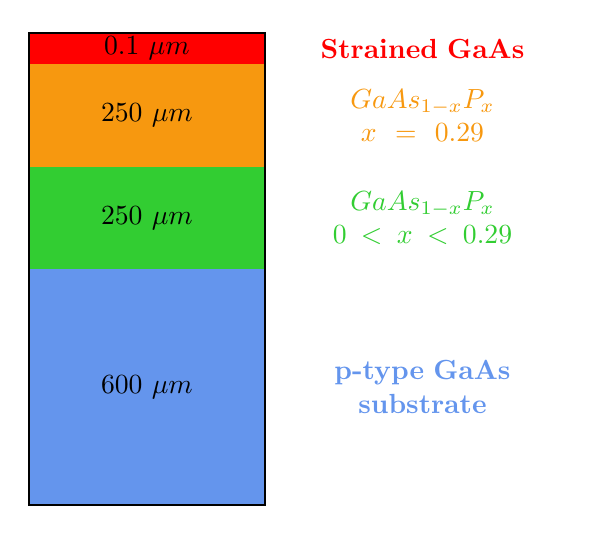
\begin{tikzpicture}
	    \tikzstyle{explain} = [align=center] 
	    \centering
	    \fill [CornflowerBlue] (0, 0) rectangle (3, 3);
	    \node at (3/2, 3/2) {\bm{$600 \ \mu m$}};
	    \node [explain, CornflowerBlue, text width=3.4 cm] at (5, 3/2) {\textbf{p-type GaAs substrate}};
	    \fill [LimeGreen] (0, 3) rectangle (3, 3+1.3);
	    \node at (3/2, 3 + 1.3/2) {\bm{$250 \ \mu m$}};
	    \node [explain, LimeGreen, text width=3.5 cm] at (5, 3+1.3/2) {\bm{$GaAs_{1-x}P_x$} \\ \bm{$0 < x < 0.29$}};
	    \fill [YellowOrange] (0, 3+1.3) rectangle (3, 3+1.3+1.3);
	    \node at (3/2, 3 + 1.3 + 1.3/2) {\bm{$250 \ \mu m$}};
	    \node [explain, YellowOrange, text width=3.5 cm] at (5, 3+1.3+1.3/2) {\bm{$GaAs_{1-x}P_x$} \\ \bm{$x = 0.29$}};
	    \fill [Red] (0, 3+1.3+1.3) rectangle (3, 6);
	    \node at (3/2, 3 + 1.3 + 1.3 + 0.4/2) {\bm{$0.1 \ \mu m$}};
	    \node [explain, Red, text width=3.5 cm] at (5, 3+1.3+1.3+0.4/2) {\textbf{Strained GaAs}};
	    \draw [thick] (0, 0) rectangle (3, 6);
	    \label{fig:excitation-a}
	\end{tikzpicture}
    \end{subfigure}
    \hfill
    \begin{subfigure}[b]{0.49\textwidth}
	\centering
	\begin{tikzpicture}
	    \begin{axis}[axis lines=middle,
		xmin=0, xmax=8,
		ymin=0, ymax=7,
		xlabel={\large $m_j$},
		ylabel={\large$E$},
		xlabel style={above},
		xtick=\empty,
		ytick=\empty,
		]
		\draw [/pgfplots/every inner y axis line, draw=black] (6.5,0) -- (6.5, \pgfkeysvalueof{/pgfplots/ymax}) node [below right] {\large J}; 
		\draw [draw=Violet, line width=2pt] (1.25,\yone) -- (2.25, \yone) node [midway, below, Violet] {\textbf{-1/2}};
		\draw [draw=Violet, line width=2pt] (4.25,\yone) -- (5.25, \yone) node [midway, below, Violet] {\textbf{+1/2}};
		\draw [draw=OliveGreen, line width=2pt] (0.5,\ytwo) -- (1.5, \ytwo) node [midway, below, OliveGreen] {\textbf{-3/2}};
		\draw [draw=OliveGreen, line width=2pt] (2,\ytwo-0.5) -- (3, \ytwo-0.5) node [midway, below, OliveGreen] {\textbf{-1/2}};
		\draw [draw=OliveGreen, line width=2pt] (3.5,\ytwo-0.5) -- (4.5, \ytwo-0.5) node [midway, below, OliveGreen] {\textbf{+1/2}};
		\draw [draw=OliveGreen, line width=2pt] (5,\ytwo) -- (6, \ytwo) node [midway, below, OliveGreen] {\textbf{+3/2}};
		\draw [draw=Blue, line width=2pt] (2,\ythree) -- (3, \ythree) node [midway, above, Blue] {\textbf{-1/2}};
		\draw [draw=Blue, line width=2pt] (3.5,\ythree) -- (4.5, \ythree) node [midway, above, Blue] {\textbf{+1/2}};
		\node [Violet, right] at (6.7, \yone-0.1) {\large\bm{$P_{1/2}$}};
		\node [OliveGreen, right] at (6.7, \ytwo-0.1) {\large\bm{$P_{3/2}$}};
		\node [Blue, right] at (6.7, \ythree-0.1) {\large\bm{$S_{1/2}$}};

		\draw [-stealth, Red, line width=2pt] (1, \ytwo) -- (2.5, \ythree) node [above, midway, sloped] {\bm{$\sigma^+$}};
		\draw [-stealth, YellowOrange, line width=2pt] (5.5, \ytwo) -- (4, \ythree) node [above, midway, sloped] {\bm{$\sigma^-$}};
	    \end{axis}
	\end{tikzpicture}
	\label{fig:excitation-b}
    \end{subfigure}
    \caption{Strained GaAs}
\end{figure}

%%%%%%%%%%%%%%%%%%%%%%%%%%%%%%%%%%%%%%%%%%%%%%%%
\subsection{Polarization Control}
\begin{itemize}
    \item Helicity Correlated Beam Asymmetry (HCBA) is the most largest false
	asymmetry to the parity-violating asymmetry
    \item It arises from the beam difference (intensity, position ...) between two helicity states from the injector
    \item A well-control of the electron source configuration can help suppress the effect of HCBA
    \item The dominant part is the Polarization Induced Transport Asymmetry (PITA) effect
\end{itemize}
\begin{figure}[h!]
    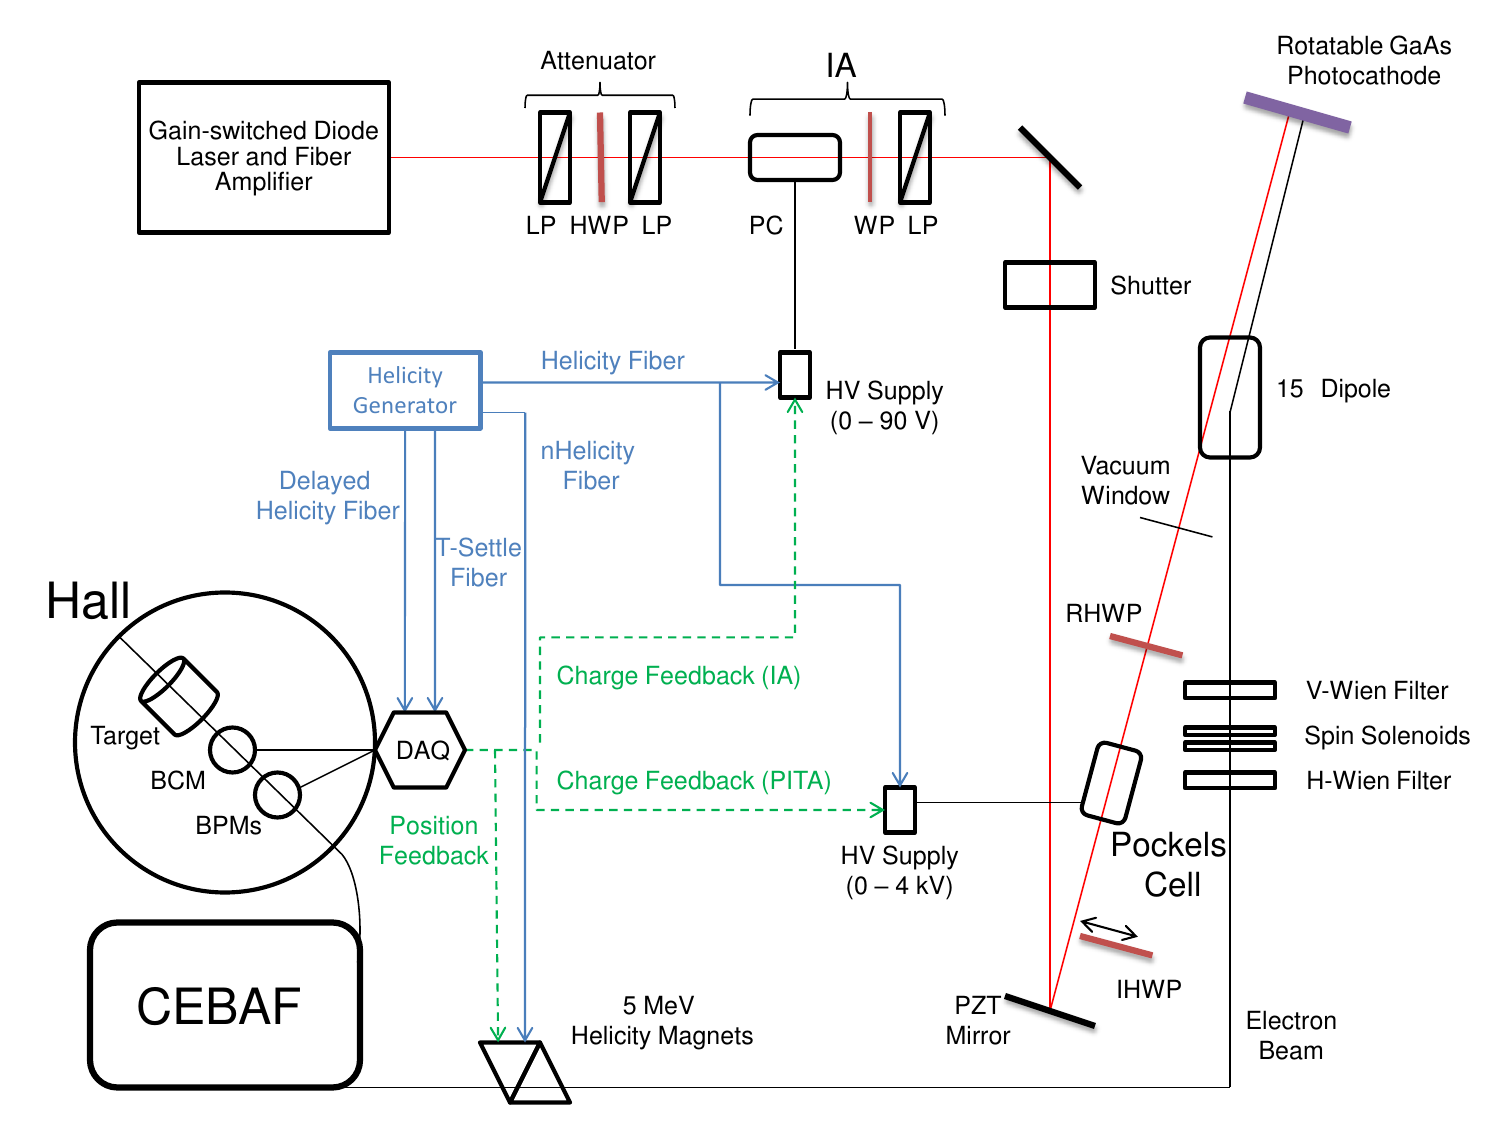
\includegraphics[width=\linewidth]{injector}
\end{figure}

\begin{figure}[h!]
    \begin{tikzpicture}
	\tikzstyle{explain} = [align=center] 
	\begin{scope}
	    \node[anchor=south west, inner sep=0] (image) at (0, 0)
	    {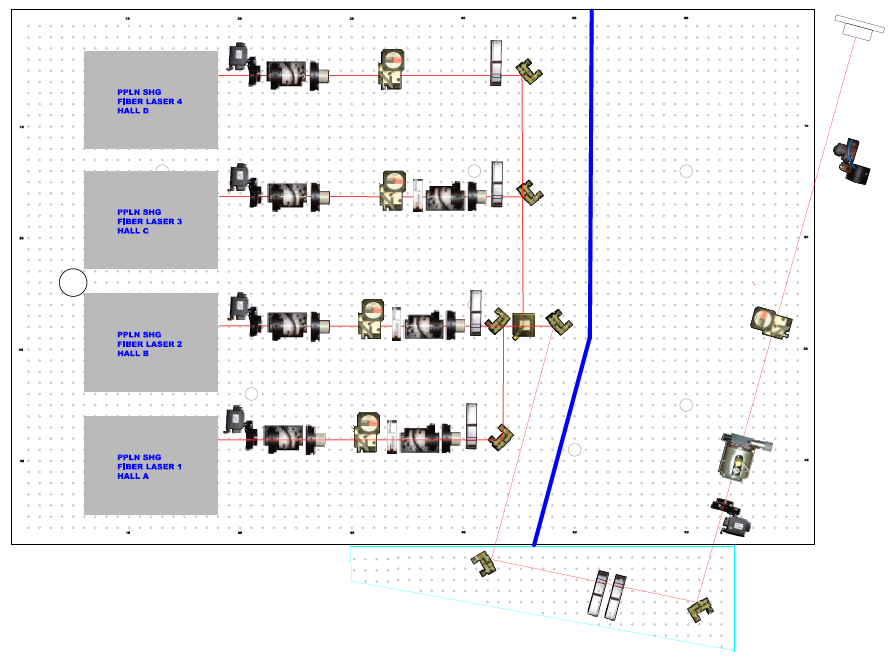
\includegraphics[width=\linewidth]{laser_table}};
	    \begin{scope}[x={(image.south east)},y={(image.north west)}]
		\node [blue,ultra thick] at (0.06,0.3) {\textbf{A}};
		\node [blue,ultra thick] at (0.06,0.49) {\textbf{B}};
		\node [blue,ultra thick] at (0.06,0.67) {\textbf{C}};
		\node [blue,ultra thick] at (0.06,0.85) {\textbf{D}};

		\node [blue,ultra thick] at (0.47,0.39) {\textbf{IA}};
		\node [blue,ultra thick] at (0.47,0.56) {\textbf{IA}};
		\node [blue,ultra thick] at (0.5,0.75) {\textbf{IA}};

		\node [red] at (0.75,0.23) {\textbf{IHWP}};
		\node [explain,red] at (0.76,0.33) {\textbf{Pockels } \\ \textbf{Cell}};
		\node [red] at (0.8,0.51) {\textbf{RHWP}};
		\node [explain,red] at (0.88, 0.96) {\textbf{Beamline} \\ \textbf{vaccum} \\ \textbf{window}};
	    \end{scope}
	\end{scope}
    \end{tikzpicture}
\end{figure}
\begin{comment}
    1. what's the beam polarization before the Pockels cell? linearly or circularly
    polarized?
\end{comment}

The following components in the injector help to control the beam polarization:
\begin{itemize}
    \item Intensity Attenuator (IA): equalize beam intensity acroos helicity states
    \item Insertable Half-Wave Plate (IHWP): slow control, flip circular polarization
    \item Pockels Cell (PC): a crystal with birefringence proportional to the applied
	electric field, it is able to convert the linearly polarized light into
	circularly polarized light. Based on Pockels effect, reversing the high voltage reverses
	the birefringence of the crystal and therefore the helicity
    \item Rotatable Half-Wave Plate (RHWP): equalized any residual linear polarization,
	establish a QE independent of helicity
    \item Two Wien filters (vertical and horizontal) and solenoid magnets are 
	used to set the spin alignment so that the electron spin is longitudinal 
	at the target
\end{itemize}

\begin{figure}[h!]
    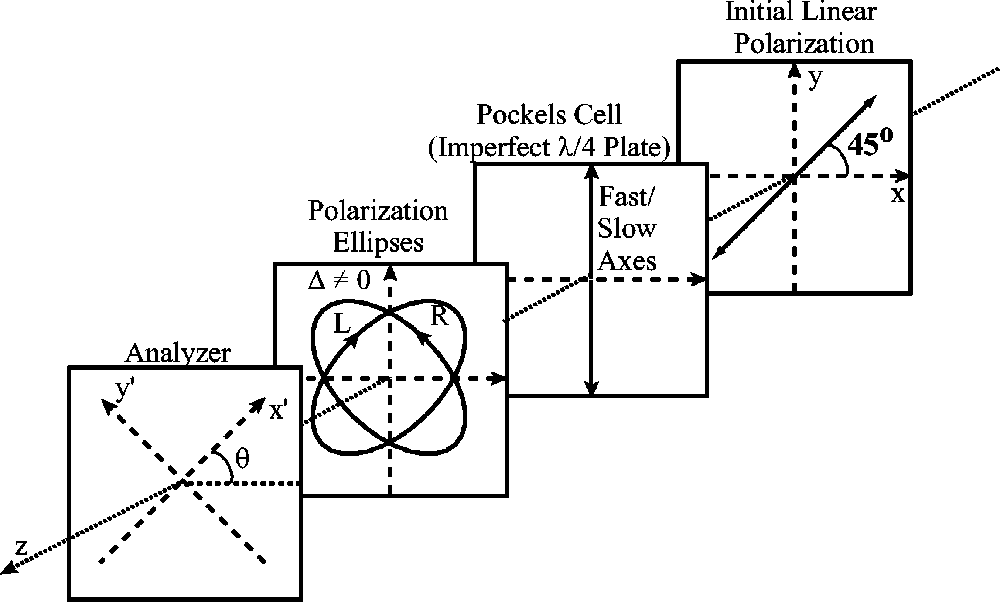
\includegraphics[width=0.7\linewidth]{PC_phase_shift}
    \caption{Phase shift by going through the PC}
\end{figure}

\begin{equation*}
    \begin{gathered}
	\delta^R = -\left(\frac{\pi}{2} + \alpha \right) - \Delta \\
	\delta^L = +\left(\frac{\pi}{2} + \alpha \right) - \Delta
    \end{gathered}
\end{equation*}

To first order:
\begin{equation*}
    \begin{gathered}
    \CA_{I} = \frac{I^R - I^L}{I^R + I^L} = -\frac{\epsilon}{T}[\Delta\cos(2\theta)]	\\
    \end{gathered}
\end{equation*}
\bigskip
\begin{itemize}
    \item $\Delta$: antisymmetric offset phase shift in PC
    \item $\epsilon/T \ (<<1)$: ``analyzing power'', $\epsilon = T_{x'} - T_{y'}$ $T = T_{x'} + T_{y'}$
    \item $\theta$: the angle between the PC's fast axis and the $x'$ transmission axis of the downstream analyzer
\end{itemize}

Considering other optical components downstream the PC:
\begin{equation*}
    \CA_{I} = -\frac{\epsilon}{T}[\cos(2\theta) \cdot (\Delta - \Delta^0)]
\end{equation*}
\begin{itemize}
    \item $\Delta^0$: offset phase shift introduced by residual birefringence in the PC and other optical components
\end{itemize}

%%%%%%%%%%%%%%%%%%%%%%%%%%%%%%%%%%%%%%%%%%%%%%%%
\subsection{Polarimeters}
We have 2 polarimeters to measure the polarization: the Compton polarimeter and
the Moller polarimeter. While being more accurate, the Moller polarimeter makes
invasive measurement, so we rely on the less accurate but non-invasive Compton
polarimeter for daily monitor of the beam polarization.

%%%%%%%%%%%%%%%%%%%%%%%%
\subsubsection{Compton Polarimeter}
The Compton polarimeter is non-invaisve, therefore it
operates all the time along data taking to monitor the beam polarization. The
Compton polarimeter locates at the entrance to hall A (about 20 m upstream the 
target chamber), using the elastic scatter between polarized photon and electron
to measured the polarization of the electron beam. As shown in fig \ref{fig:compton_pol},
when the compton polarimeter is on, the electron beam will be bent into the 
Compton chicane to interact with the polarized photons. The photon energy is 
2.33 eV and the crossing angle is $23.5^\circ$. The scattered photons will be
detected by the photon detector right of the interaction region, while the
electron beam will be bent back to the beam pipe to bombar the target. Due to
interaction with photons, the scattered electrons will be less energetic than
the incoming ones. So under the same dipole field, the scattered electrons will
be bent more than the non-interacting ones, as shown by the red dash line. This 
seperation allow us to measure the scattered electrons, together with measurement
of scattered photons, we can identify and scattering asymmetry and then the polarization
of the electron beam.
\begin{equation*}
    \CA_{\text{th}} = \frac{\sigma_{\Rightarrow}^{R} - \sigma_{\Rightarrow}^{L}}{\sigma_{\Rightarrow}^{R} + \sigma_{\Rightarrow}^{L}}  \qquad
    \CA_{\text{exp}} = \CP_{e}\CP_{\gamma}\CA_{\text{th}} = \frac{N_{\gamma}^R - N_{\gamma}^L}{N_{\gamma}^R + N_{\gamma}^L}
\end{equation*}
The Compoton polarimeter is able to achieve a 1\% overall absolute systemtatic
uncertainty.
\begin{figure}[h!]
    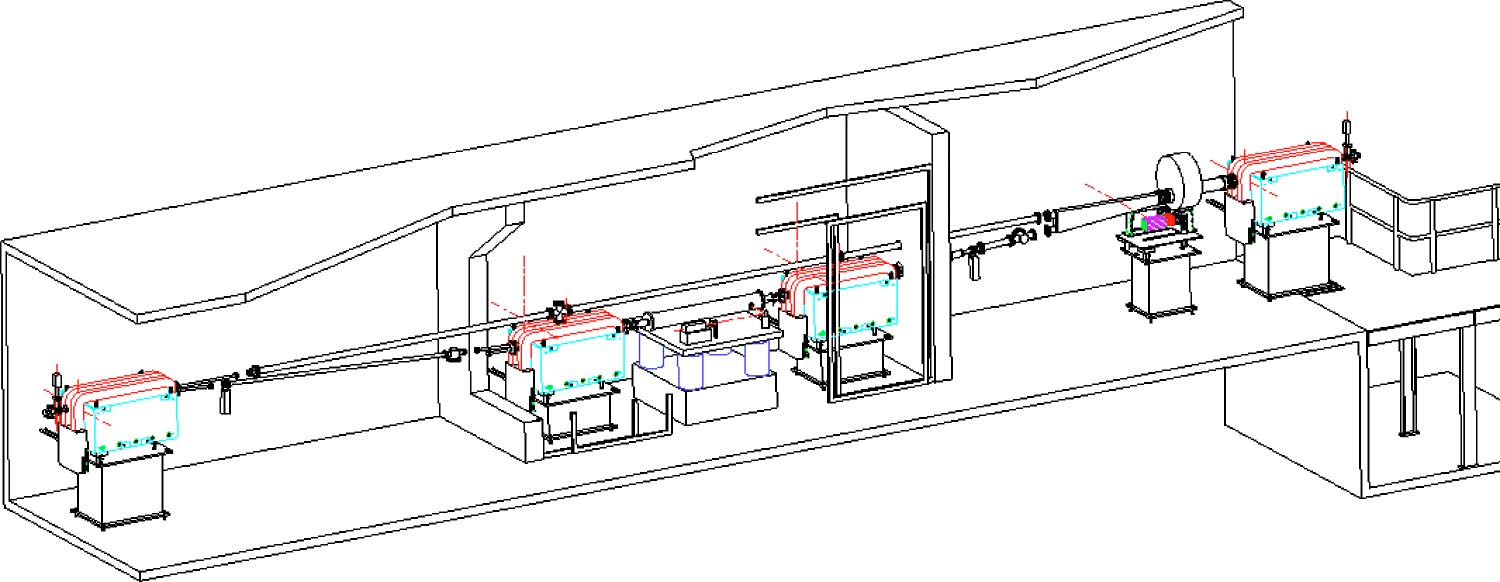
\includegraphics[width=0.49\linewidth]{Compton_setup}
    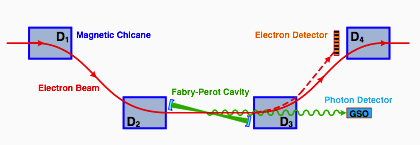
\includegraphics[width=0.49\linewidth]{Compton_beam_path}
    \caption{Left: Compton chicane; Right: Schematic plot of electron/photon 
    scattering} 
    \label{fig:compton_pol}
\end{figure}

%%%%%%%%%%%%%%%%%%%%%%%%
\subsubsection{Moller Polarimeter}
The Moller polarimeter uses elastic electron-electron scattering to measure the
asymmetry due to different beam polarizations. Since this is a pure QED process,
its cross section is well understood and easily calculable to high order:
\begin{equation*}
    \frac{d\sigma}{d\Omega} = \left( \frac{d\sigma_0}{d\Omega} \right) [ 1 + P_b \cdot P_t \cdot A_{ZZ}(\theta)]
\end{equation*}
Where $\frac{d\sigma_0}{d\Omega} = \left( \frac{\alpha(4 - \sin^2\theta)}{2m_e\gamma\sin^2\theta }\right)^2$ is the unpolarized cross section and $A_{zz}(\theta)$ is the analyzing power, 
in CoM frame, $A_zz(\theta) = -\sin^2\theta \frac{8 - \sin^2\theta}{(4-\sin^2\theta)^2}$.
When $\theta_{CoM} = 90^\circ$, $A_{zz}$ is maximized to be $-\frac{7}{9}$.
$P_b (P_t)$ is the polarization of beam (target). The polarized target electrons
are provided by magnetized Fe-alloy foil, a strong (FIXME: how much) magnetic 
field is required to polarized the target electrons. The scattered electrons will
be separated by quadrupole or septum magnet, and then collected by electron 
detectors. Because Moller measurement is invasive, it happens about every 10 days.
\begin{figure}[h!]
    \centering
    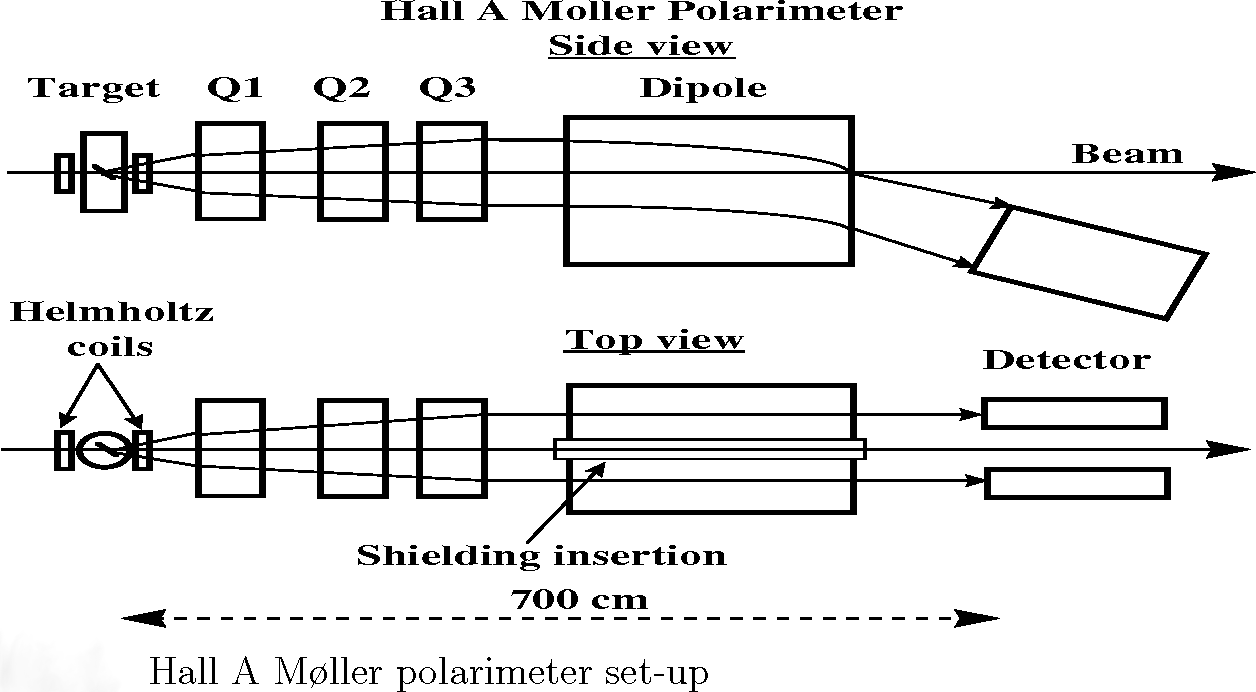
\includegraphics[width=0.7\linewidth]{moller_setup}
\end{figure}

%%%%%%%%%%%%%%%%%%%%%%%%%%%%%%%%%%%%%%%%%%%%%%%%
\section{Target}
As tiny as the neutron skin thickness, to measure it relatively accurate, the
larger it is, the better our measurement will be. So the target elements should
have a large neutron excess. So \Pb (\Ca) is chosed for PREX-II (CREX). Some
bonus from the choice are:
\begin{itemize}
    \item Both are doubly-magic nuclei, which means they are stable than their
	isotope
    \item They are spin-0, no need to worry about the target polarization
    \item Their first inelastic states are large, 2.6 MeV for \Ca, which helps
	to reduce background from inelastic scattering
    \item Both are heavy nuclei, which reduces recoiling effect and help
	to achive low $Q^2$
\end{itemize}

In addition to the production targets, we had other targets to ensure our 
understanding of the spectrometer optics. For example, we have Carbon Hole target
to identify the beam position; there is Carbon target to measure the scattering
rate of \C. A water target in the $45^\circ$ ladder helps to calibrate the 
scattering angle, etc.

\begin{figure}[h!]
    \centering
    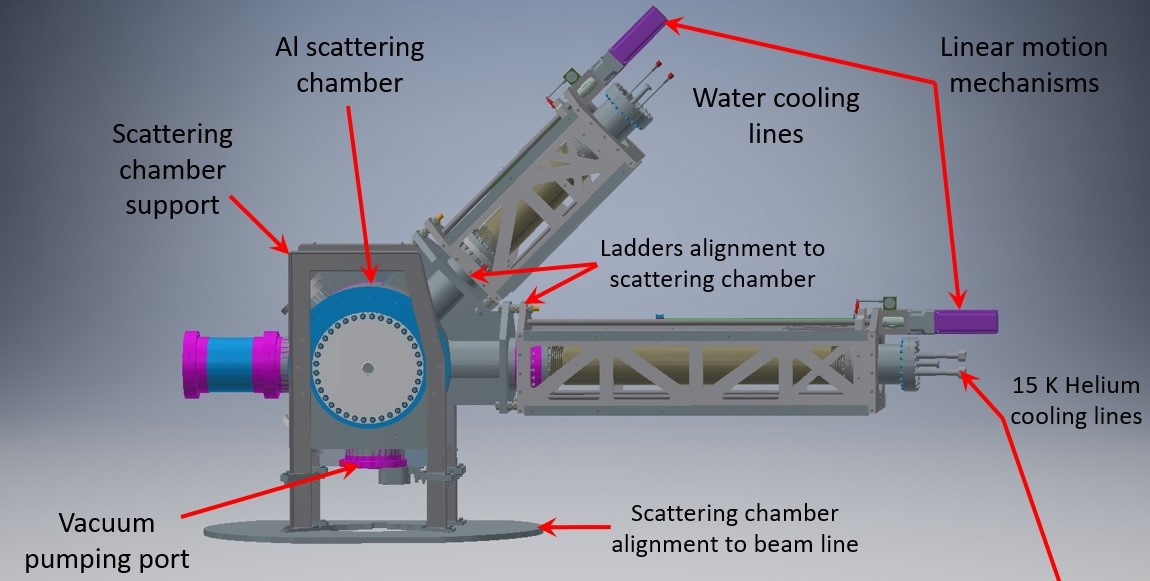
\includegraphics[width=\linewidth]{target_1}
\end{figure}

Lessens learn from PREX-I (2010): over a few days of running, the incident
electron beam degraded the Pb target; therefore we have multiple targets in
PREX-II. Although the soft metal was cooled to 20 K, it still melted and 
deformed under the beam's bombardment. Small nonuniformities in the target 
thickness vary the scattering rate, and over the course of the experiment they 
eventually generated enough noise to swamp the tiny weak-scattering signal.

The PREX researchers found that they could significantly reduce the sensitivity 
to target-thickness variations by synchronizing the scattering-rate measurements 
with the back-and-forth motion of the beam as it sampled different areas on the target. 
That technique was used for their second run in 2019, and they made extra targets 
so each one could be switched out as soon as it showed signs of degradation.

\subsection{Target Cooling}

%%%%%%%%%%%%%%%%%%%%%%%%%%%%%%%%%%%%%%%%%%%%%%%%
\section{Raster}
The non-uniformity of the thickness of target foils due to electron bambarbment, 
if not corrected, will caused large noise to our asymmetry measurement. 
Generally, the central beam area will become thinner while the outer area will 
become thicker, Actually, this is how we see the status of a target foil and decide
to replace a target foil if the measured asymmetry width increase significantly.

%%%%%%%%%%%%%%%%%%%%%%%%%%%%%%%%%%%%%%%%%%%%%%%%
\section{Collimator and Sieve}
The collimator box is ??? downstream the target chamber, which is critical for
controlling the radiation. Water cooled Tungsten with Copper jacket, 2 KW cooling
is required in collimator.

%%%%%%%%%%%%%%%%%%%%%%%%%%%%%%%%%%%%%%%%%%%%%%%%
\section{Septum}
The septum magnet is required to bridge the scattered electrons at small angle
into the HRS. As said before, the designed scattering angle is about $5^\circ$
while the smallest angle that HRS can reach is $12.5^\circ$, so we need the septum
magnet to guide the scattered electrons into HRS. 

The septum magnets are normal conducting magnets that consist of 3 coils, 
by applying large current, it will produce a
strong magnetic field (up to $\sim 1 \ T$ in the central region). A septum beampipe
will connect the upstream collimator box and the downstream HRS vacuum pipe.

\begin{figure}[h!]
    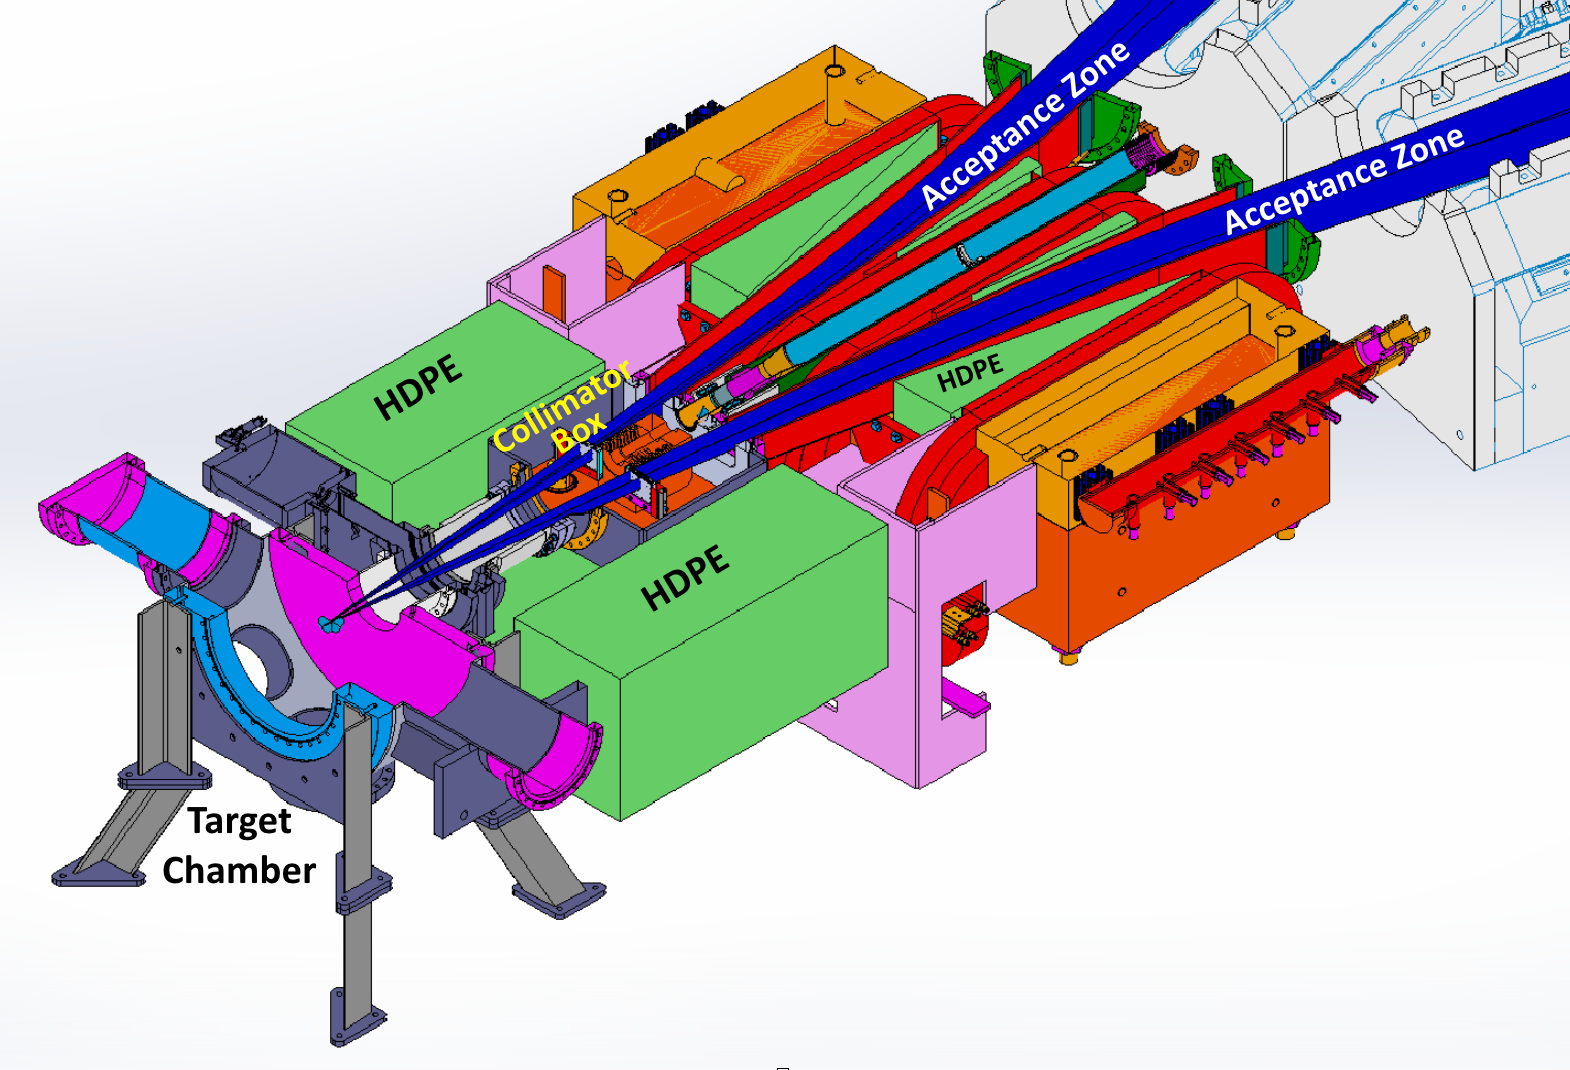
\includegraphics[width=0.52\linewidth]{septum}
    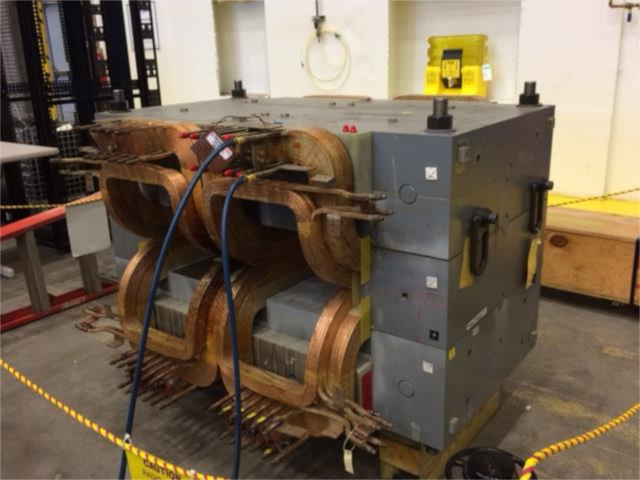
\includegraphics[width=0.46\linewidth]{septum_real}
\end{figure}

%%%%%%%%%%%%%%%%%%%%%%%%%%%%%%%%%%%%%%%%%%%%%%%%
\section{High Resolution Spectrometer (HRS)}
As its names implies, the high resolution capability of the spectrometer helps
us to reject most of inelastic electrons, leaving us a relative clean data with
very small background from inelastic scattering. The HRS consists of 3 quadrupoles 
and one dipole in each arm, the quadrupoles magnetic field is around $0.2 \ T$,
while the dipole magnetic field will reach as high as $0.4 \ T$.
the collimator at the Q1 entrance defines the acceptance shape.
\begin{figure}[h!]
    \centering
    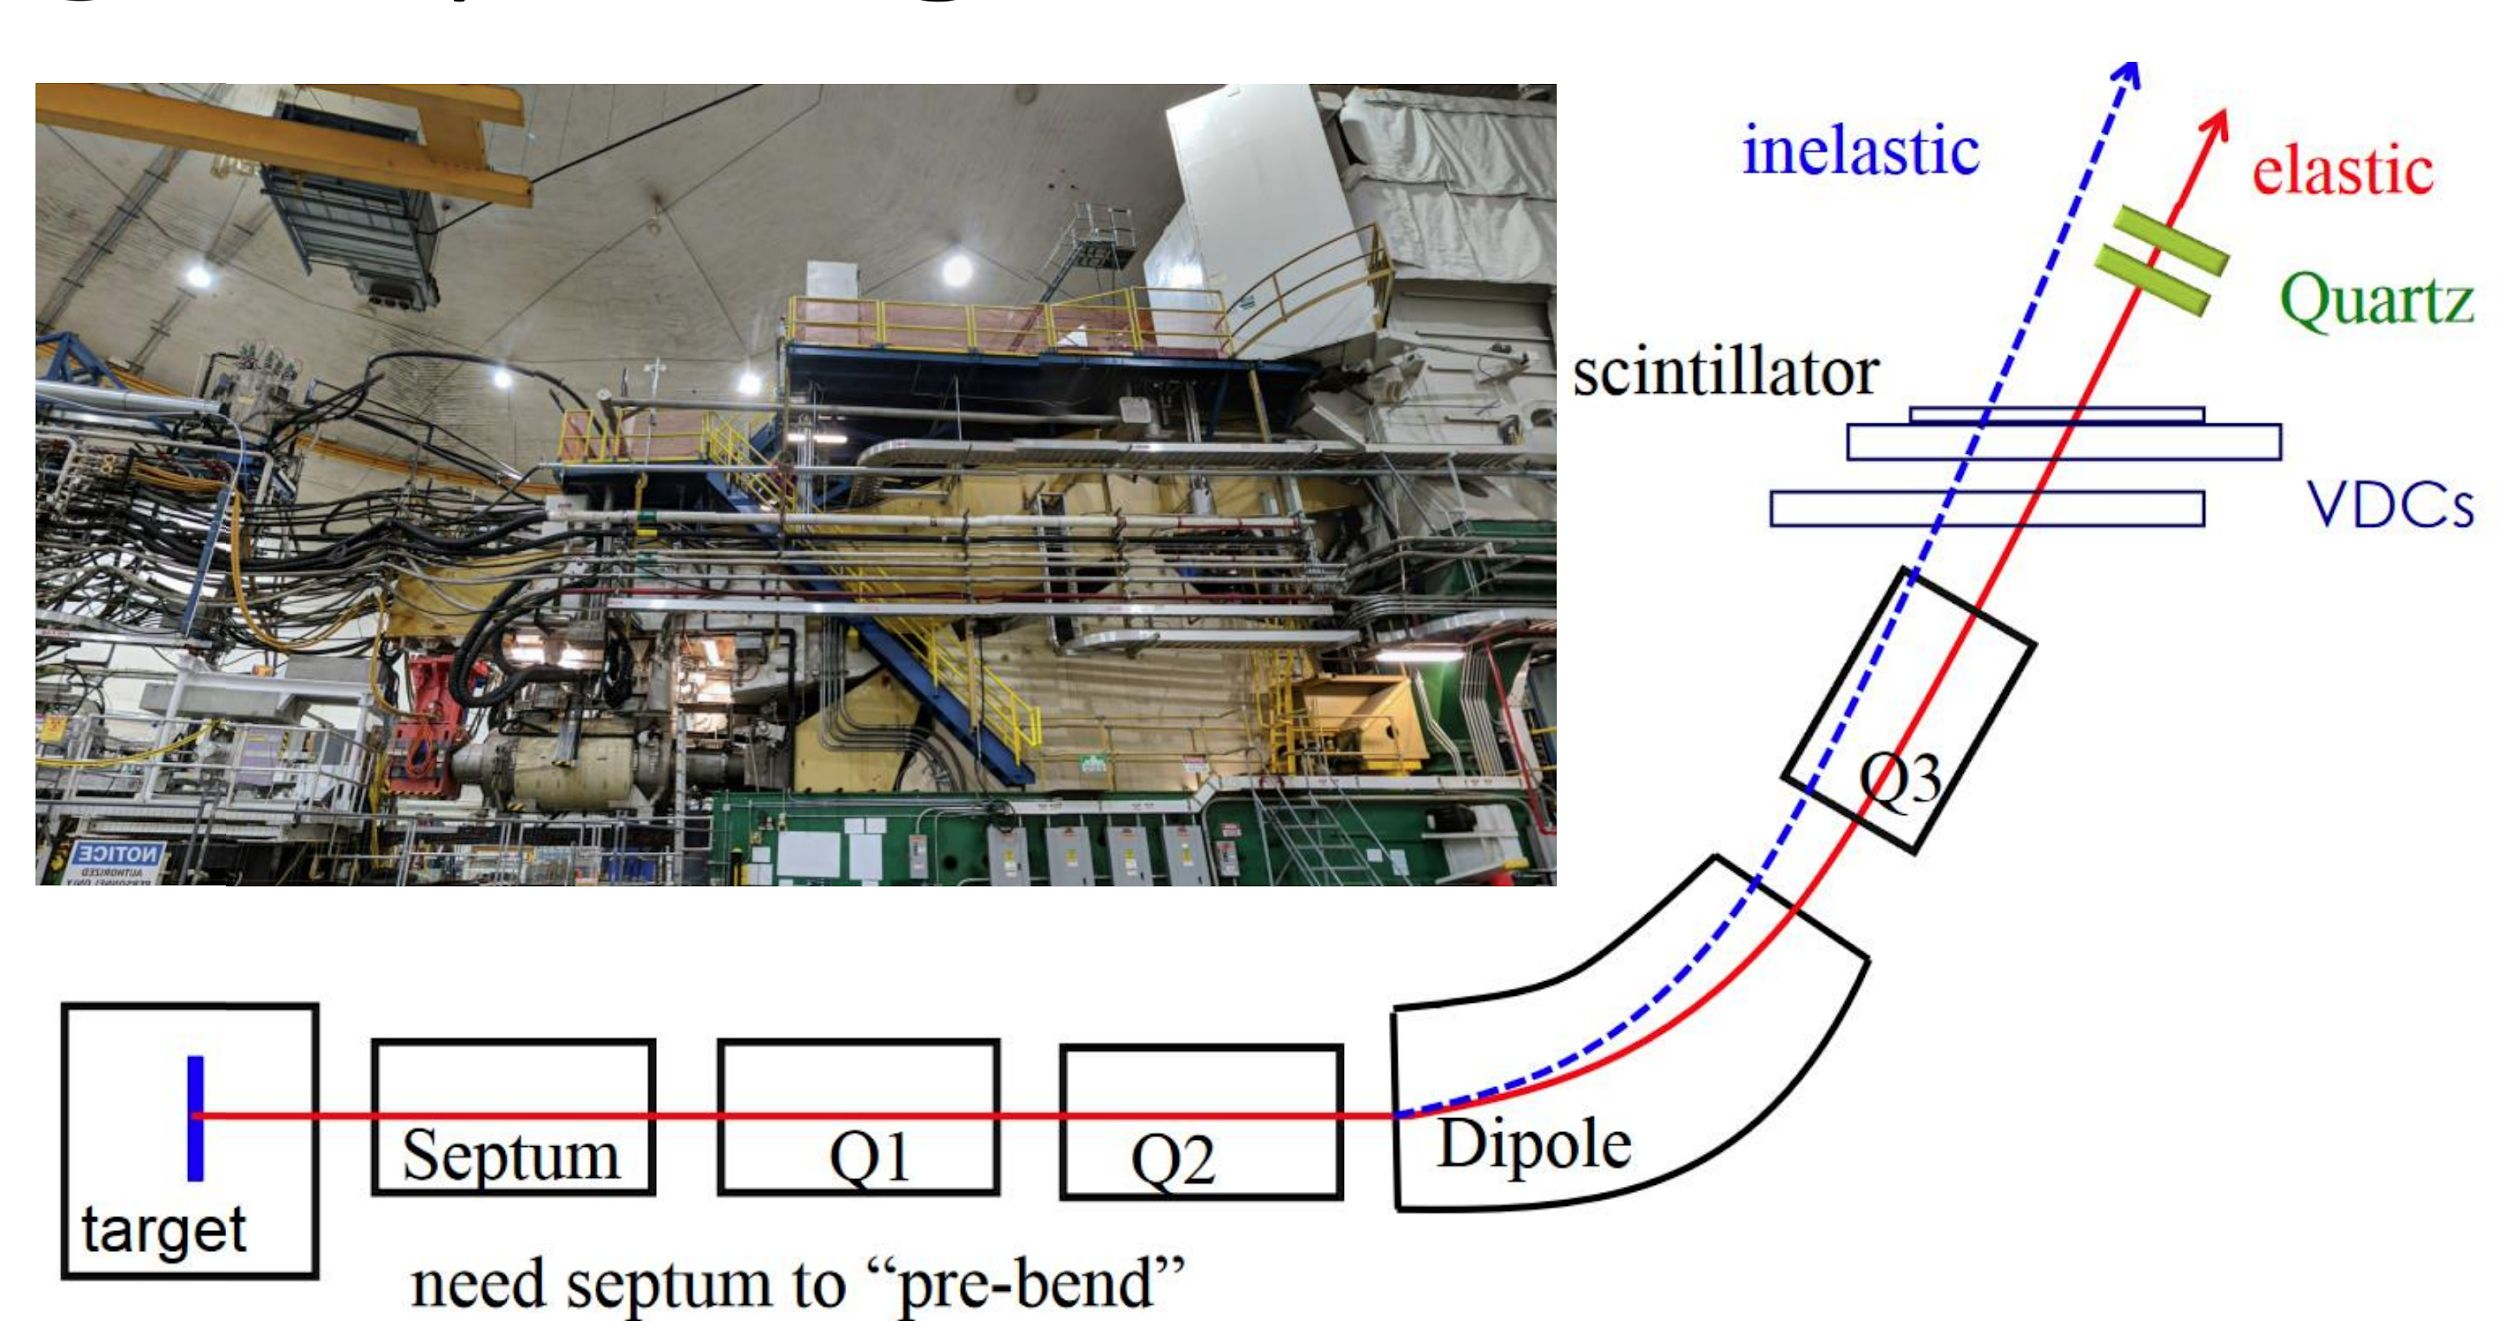
\includegraphics[width=0.8\linewidth]{HRS}
\end{figure}

%%%%%%%%%%%%%%%%%%%%%%%%%%%%%%%%%%%%%%%%%%%%%%%%
\section{Detector}

\section{Data AcQuisition (DAQ)}
We use to pseudo random number generator to decide the helicity pattern, which
will trigger the data taking of both detectors and monitors. DAQ will read data
from PCs, BPMs, BCMs and detectors, which will then be digitalized by a 18 digits
ADC. In one helicity window, they will sample ??? times, which will be grouped
into 4 blocks. The sum of the 4 blocks was what we got.

The integrated response of each detector and beam monitor was collected and sampled 
by a custom 18-bit ADC for each helicity window.
%%%%%%%%%%%%%%%%%%%%%%%%
\subsection{Beam Position Monitor (BPM) and Beam Current Monitor (BCM)}
Hall A resolution

\begin{itemize}
    \item Microwave Cavity BPM and BCM
    \item Stripline Electrode Electronic (SEE) BPM and BCM
    \item Cross check, and unfold beam fluctuation noise from instrumentation noise
\end{itemize}

%%%%%%%%%%%%%%%%%%%%%%%%%%%%%%%%%%%%%%%%%%%%%%%%
\section{Beam Modulation}
It is very important for PVES to control the systematic uncertainty, especially
the one from beam fluctuation (HCBA). Ideally, the electrons bunches with opposite
polarization should have exactly the same internsity and energy, hitting the target 
at the same place with the same angle, which is obviously impossible in reality. 
So we need to correct the false asymmetry introduce by the beam fluctuation. There are a
few methods to do the correction, one of them is the so called Beam modulation.
The idea is to introduce man-made fluctuations to the beam through the 
modulation system, then we can measure the changes in monitors and detectors 
to find the sensitivities of detectors to changes in energy, position and angle,
which will be used to correct the measured asymmetry.

The beam modulcation system lies in Beam Switch Yard area right after existing 
the CEBAF, it consists of 7 air-core coils and an energy vernier, the total 
number of 8 coils provides a redudancy w.r.t. the free number of degrees 
of beam phase space, making sure to cover all beam phase space at target.  
These coils (vernier) are driven by a VME-DAC, which in turns is controlled by the parity DAQ.
It takes 4.267 s for each coil (vernier) to modulate the beam, a whole 
modulation cycle takes $85.68 \ s$ ($\sim 1$ beam modulation every 10 mins during
data taking). For the position and angle modulation, the beam diplacement will
be $0.3-0.5\ \mu m$ and energy vernier will result in a beam diplacement of $0.75 \ mm$
\begin{figure}[h!]
    \centering
    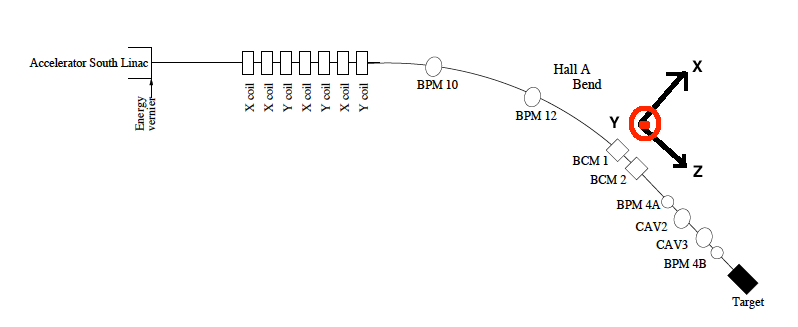
\includegraphics[width=0.49\linewidth]{bmw_setup}
    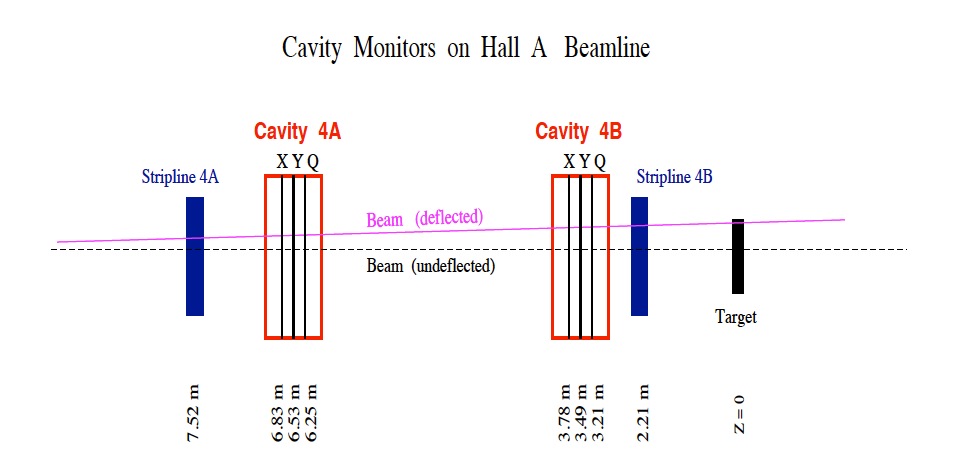
\includegraphics[width=0.49\linewidth]{bmw_modulated_beam}
\end{figure}

